\PassOptionsToPackage{unicode,pdfusetitle}{hyperref}
\PassOptionsToPackage{hyphens}{url}

\documentclass[twoside]{article}
\usepackage[a4paper,includeheadfoot,top=0cm,bottom=0.2cm,left=1.5cm,right=0.2cm]{geometry}
\usepackage{amsmath,amssymb}
\usepackage{fontspec}
\usepackage[russian]{babel}
\usepackage{microtype}
\usepackage{parskip}
\usepackage{xcolor}
\definecolor{navy}{RGB}{0,0,128}
\setmainfont{Noto Serif}
\setsansfont{Monitorica}
\setmonofont{Noto Sans Mono}
\newfontfamily\headingfont{Operation Napalm}
\newfontfamily\titlefont{Magnolia Script}
\usepackage{titlesec}
\titleformat{\section}{\headingfont\color{navy}\Large}{\thesection}{1em}{}[\titlerule]
\titleformat{\subsection}{\headingfont\color{navy}\large}{\thesubsection}{1em}{}
\titleformat{\subsubsection}{\headingfont\color{navy}\normalsize}{\thesubsubsection}{1em}{}
\titleformat{\paragraph}{\headingfont\color{navy}\normalsize}{\theparagraph}{1em}{}
\titleformat{\subparagraph}{\headingfont\color{navy}\normalsize\itshape}{\thesubparagraph}{1em}{}
\usepackage{multicol}
\usepackage{array}
\usepackage{background}
\usepackage{wallpaper}
\usepackage{tabularray}
\usepackage{tblr-extras}
\usepackage{multirow}
\usepackage{makecell}
\usepackage{calc}
\usepackage{rotating}
\usepackage{caption}
\usepackage{capt-of}
\usepackage{titletoc}
\usepackage{graphicx}
\usepackage{wrapfig}
\UseTblrLibrary{booktabs,caption,babel}
\makeatletter
\def\maxwidth{\ifdim\Gin@nat@width>\linewidth\linewidth\else\Gin@nat@width\fi}
\def\maxheight{\ifdim\Gin@nat@height>\textheight\textheight\else\Gin@nat@height\fi}
\makeatother
\setlength{\emergencystretch}{3em}
\providecommand{\tightlist}{
  \setlength{\itemsep}{0pt}\setlength{\parskip}{0pt}}
  \providecommand{\fillinline}[1]{
  \leavevmode\leaders\hbox to 0.5556em{\hss.\hss}\hfill\kern0pt}
\setcounter{secnumdepth}{5}
\setcounter{tocdepth}{3}
\titlecontents{section}[0em]{}{\headingfont\Large\makebox[1.3em][l]{\thecontentslabel}}{}{\titlerule*[0.8pc]{.}\contentspage}
\titlecontents{subsection}[0em]{}{\headingfont\large\makebox[2.1em][l]{\thecontentslabel}}{}{\titlerule*[0.8pc]{.}\contentspage}
\titlecontents{subsubsection}[0em]{}{\headingfont\makebox[3.2em][l]{\thecontentslabel}}{}{\titlerule*[0.8pc]{.}\contentspage}
\titlecontents{paragraph}[0em]{}{\headingfont\small\makebox[4.2em][l]{\thecontentslabel}}{}{\titlerule*[0.8pc]{.}\contentspage}
\titlecontents{subparagraph}[0em]{}{\headingfont\footnotesize\makebox[5.0em][l]{\thecontentslabel}}{}{\titlerule*[0.8pc]{.}\contentspage}
\usepackage{bookmark}
\IfFileExists{xurl.sty}{\usepackage{xurl}}{}
\urlstyle{same}
\hypersetup{
  hidelinks
}

\captionsetup{labelfont={it,color=navy},textfont={it,color=navy},justification=centering}
\captionsetup[table]{hypcap=false}
\captionsetup[figure]{hypcap=false}
\addto\extrasrussian{
  \def\figurename{Схема}
  \def\tableautorefname{Таблица}
  \def\figureautorefname{Схема}
  \def\sectionautorefname{Раздел}
  \def\subsectionautorefname{Подраздел}
  \def\subsubsectionautorefname{Параграф}
  \def\paragraphautorefname{Абзац}
  \def\pageautorefname{Страница}
  \def\equationautorefname{Формула}
}

\title{Мир и процветание}
\newcommand{\siteurl}{https://vk.com/playingwar}
\author{Никита Макаров}

\begin{document}

\begin{titlepage}
\backgroundsetup{
  scale=1,
  angle=0,
  opacity=1,
  position={current page.center},
  contents={
\includegraphics[width=\paperwidth,height=\paperheight,clip]{media/pap_players_book/image2.png}}
}

\begin{center}
\vspace*{2cm}

{\color{purple}\fontsize{48}{56}\titlefont\selectfont{Мир и процветание}}

\vspace{0.5cm}

{\color{teal}\fontsize{32}{40}\titlefont\selectfont{Книга мастера}}

\vfill

{\color{white}\Large\textbf{Никита Макаров}}

{\color{white}\href{\siteurl}{\textbf{\MakeUppercase{\siteurl}}}}

{\color{white}\textbf{Санкт-Петербург}}

\end{center}
\end{titlepage}

\clearpage

\backgroundsetup{
  scale=1,
  angle=0,
  opacity=1,
  position={current page.center},
  contents={\TileWallPaper{1cm}{1cm}{media/common/image1.jpg}}
}

\begin{multicols}{2}
\raggedcolumns{}

\renewcommand{\contentsname}{Содержание}
\pagestyle{empty}
\tableofcontents
\clearpage
\pagestyle{plain}

\section{Введение}\label{intro}

Вашему вниманию предлагается сценарий к игре Контракт.

Действие происходит в наше время в альтернативной реальности, где
государства передают управление военизированными операциями крупным
международным компаниям.

Компания ``Мир и процветание'' заключает договор с правительством Белиза о
предоставлении услуг в области охраны правопорядка и обороны страны.
Договор предусматривает поэтапный переход функций от армии и полиции к
компании ``Мир и процветание'' с последующим расформированием
государственных структур, но для этого компании предстоит доказать свою
эффективность в течение переходного периода.

Не все довольны этой ситуацией. Некоторые кадровые офицеры армии и
полиции Белиза опасаются, что потеряют своё влияние, доход и положение в
обществе. Националисты из разных слоёв общества воспринимают приход
транснациональной компании как нарушение суверенитета и готовы
противостоять ей любыми средствами. Некоторые просто пользуются
ситуацией и возможностями, открывающимися из-за неизбежных накладок во
время переходного периода, для личного обогащения.

Компания ``Мир и процветание'' нанимает людей для работы в Белизе через
сеть своих офисов в разных странах.

\section{Краткий обзор}\label{overview}

Персонажи игроков подписывают контракт с компанией ``Мир и процветание'',
проходят подготовку в учебном центре компании и затем отправляются в
Белиз.

В учебном центре вместе с персонажами игроков обучается Леонард Кучин,
который не обладает достаточной для этой работы психоэмоциональной
устойчивостью, что заканчивается трагично.

Только прибыв в Белиз, персонажи игроков становятся невольными
свидетелями жестокого нападения на вооружённых оперативников <<Мира и
процветания>>. Это событие является серьёзной угрозой для бизнеса
компании.

Персонажи игроков располагаются на базе ``Мира и процветания'' в городе
Бельмопан и становятся оперативниками.

В это же время в Белиз прибывает агент ЦРУ США. Управление по борьбе с
наркотиками США охотится за руководством наркокартеля, распространяющего
наркотики в США. Осуществляя мониторинг подозрительных финансовых
операций, возможно, связанных с торговлей наркотиками, оно направило
запрос в правительство Белиза об одном из трансграничных платежей между
счетами Рика Вальса и Хуана Эстебана Карреры, на что пришла странная
отписка, что таких людей не существует. Управление по борьбе с
наркотиками решило привлечь ЦРУ для проверки информации. ЦРУ нашло
информацию о Каррере и установило, что ему принадлежат особняк и
автомастерская ``Винт и болт'' в Бельмопане.

Руководитель базы ``Мира и процветания'' Ханс Шмидт доверяет персонажам
игроков, потому что они прибыли из другой страны и заведомо не связаны с
местными группировками. Он сразу же определяет их основную задачу как
поиск виновных в нападении на машину ``Мира и процветания'' и тех, кто их
финансирует и снабжает оружием.

Ханс Шмидт знаком с бывшим офицером армии Белиза, Хуаном Эстебаном
Каррерой, который после увольнения из армии занимается нелегальной
торговлей оружием. Шмидт предполагает, что оружие поступает из армии
Белиза, но думает, что оно уходит за рубеж, в США. Также Шмидт знает,
что Виктор Кравченко, интендант ``Мира и процветания'', отвечающий за
вооружение, тоже иногда покупает оружие у Карреры, когда возникают
сложности с доставкой, а оружие или боеприпасы требуются срочно.

Хуан Эстебан Каррера покупает оружие у действующего офицера армии Белиза
Ахмеда Хассана и действительно продаёт его клиентам из других стран.

Однако, Каррера не знает, что среди его клиентов --- местный наркобарон
Энрике Вальдес (скрывающийся под псевдонимом Рик Вальс). И уж тем более
он не в курсе, что Вальдес снабжает оружием террориста-националиста
Рауля Мендосу, который считает договор правительства Белиза и <<Мира и
процветания>> предательством и хочет вернуть суверенитет Белиза, вступив
в борьбу с ``Миром и процветанием''. Но Вальдес --- не националист, он
просто опасается, что ``Мир и процветание'' возьмёт под контроль его
бизнес.

Также Каррера не знает, что Ахмед Хассан, который продаёт ему оружие,
ворует его не только непосредственно у армии Белиза, но и получает от
Алексея Смирнова, администратора и интенданта базы ``Мира и процветания''.
Алексей подкупает некоторых оперативников ``Мира и процветания'', которые
по фиктивным документам, подписанным Алексеем, получают оружие и
передают его солдатам армии Белиза, подкупленным Ахмедом Хассаном.

Ахмеду Хассану не нужна война, ему достаточно, чтобы всё оставалось как
было до прихода ``Мира и процветания''. Армия Белиза --- его дом, а
воровство оружия -- норма жизни. Он дорожит своим местом в армии Белиза,
поэтому, хоть и получает часть прибыли за счёт ``Мира и процветания'', на
самом деле хочет изгнать ``Мир и процветание'' из страны, чтобы армию
Белиза не расформировали.

И Вальдес, и Хассан связаны с бандитом Рашидом Гомесом. Вальдес
использует его, чтобы вооружать Мендосу, оставаясь в тени, а Хассан,
чтобы очернить ``Мир и процветание'' перед правительством Белиза и
выставить компанию неспособной обеспечить порядок. Хассану достаточно,
чтобы банда Рашида создавала хаос и обеспечивала недовольство общества и
правительства.

Наблюдая за автомастерской ``Винт и болт'', агент ЦРУ обнаруживает, что
она обслуживает грузовики, причём они иногда они приезжают гружёные, а
уезжают пустые, или наоборот. В ящиках -- оружие с армейской базы,
передаваемое Ахмедом Хассаном. Это оружие забирает Рашид Гомес с
помощниками и агент ЦРУ решает проследить за ним.

Ханс Шмидт решает поговорить с Хуаном Эстебаном Каррерой и
договаривается с ним о встрече. Он берёт несколько оперативников с собой
и едет на встречу с Каррерой в его особняк. Алексей Смирнов узнаёт об
этом и, опасаясь своего разоблачения, отправляет подкупленных им
оперативников ``Мира и процветания'' убить Карреру, чтобы расследование не
продвинулось. Снайпера атакуют Карреру прямо во время разговора. Шмидт
предлагает Каррере укрыться на базе ``Мира и процветания'' и тот
соглашается. Даже если снайперам не удаётся убить Карреру на месте, и
персонажи игроков сопровождают его на базу, Карреру всё равно убивают
ночью прямо на базе.

Вскоре один из патрулей ``Мира и процветания'' замечает людей, перевозящих
оружие, отслеживает их вплоть до их схрона и сообщает об этом
руководству. Это и есть группа Рашида Гомеса. Ханс Шмидт приказывает
произвести арест боевиков и направляет для этого оперативников. Сразу же
после ареста место схрона накрывает миномётный обстрел. Обстрел этот
организован армейскими наблюдателями с целью скрыть возможные улики
связи Гомеса с Хассаном.

В это время на контакт с ``Миром и процветанием'' выходит сержант армии
Белиза, который хочет работать в ``Мире и процветании'' по личным
соображениям, и в знак лояльности передаёт информацию, вскрывая схему
передачи оружия ``Мира и процветания'' Ахмеду Хассану.

В это же время Алексей Смирнов решает, что ему больше небезопасно
оставаться в Белизе, и тайно сбегает из страны. За время работы он
накопил достаточно, чтобы не держаться за компанию. Однако, перед уходом
он выполняет последнюю просьбу от Ахмеда Хассана, за что получает
хорошее вознаграждение: анонимно направляет в правительство Белиза
поддельные документы, из которых следует, что именно Ханс Шмидт продавал
оружие Хуану Эстебану Каррере.

Отношения ``Мира и процветания'' с правительством ухудшаются и достигают
критической точки: от ``Мира и процветания'' требуют свернуть деятельность
в стране в течение месяца. Никакие государственные структуры Белиза
больше не поддерживают ``Мир и процветание''.

Ханс Шмидт, тем не менее, не собирается сдаваться и решается на крайне
рискованный шаг: он приказывает своим оперативникам устроить засаду на
армейский конвой, чтобы захватить Ахмеда Хассана -- с целью допроса. Это
тайная операция, оперативники действуют так, чтобы их невозможно было
связать с компанией ``Мир и процветание''.

Хассана привозят на пустующую ферму. Шмидт допрашивает его лично -- без
лишних свидетелей, без протоколов. Он понимает: отпускать Хассана в
нынешней ситуации -- слишком опасно. Поэтому убивает его сам.

Шмидт приказывает своим оперативникам атаковать базу
националистов-террористов Рауля Мендосы, чтобы показать результат
правительству Белиза и вернуть репутацию компании ``Мир и процветание''.

На базе Рауль пытается убедить персонажей игроков перейти на его
сторону, аргументируя тем, что ни ``Мир и процветание'', ни армия, ни
текущее правительство не смогут обеспечить мир и процветание Белиза,
потому что между ними нет никакой разницы -- все они погрязли в
коррупции и беззаконии.

Рауль Мендоса --- идеалист. Он не знает, что за оружие платит Энрике
Вальдес, а само оно украдено у армии Белиза и даже у <<Мира и
процветания>> и несколько раз перепродано. Оружие попадает к Раулю через
Рашида Гомеса, который прикидывается перед Раулем мирным жителем, и у
Рауля создаётся впечатление, как будто его поддерживает народ.

Агенты ЦРУ, опираясь на оперативников ``Мира и процветания'', через
наркодилера Тайлера Дердена выходят на нарколабораторию. Там они узнают
местонахождение особняка Энрике Вальдеса, а также информацию о том, что
Вальдес вёл в лаборатории разработку биологического или генетического
оружия. В лаборатории оперативники ``Мира и процветания'' обнаруживают
огромного искусственно выращенного монстра и убивают его.

В особняке Вальдеса агенты ЦРУ арестовывают или убивают Вальдеса.

Таким образом, ``Мир и процветание'' не только полностью выигрывает Белиз,
но и получает много очков на рынке США за счёт сотрудничества с ЦРУ.

\section{Создание персонажей}\label{char-creation}

Игроки могут начать игру в разных ролях:

\begin{itemize}
\item
  как обычные наёмники;
\item
  как агент(ы) ЦРУ:

  \begin{itemize}
  \item
    в начале игры --- под прикрытием обычных наёмников;
  \item
    в ходе игры --- в любое время; в этом случае мастеру нужно продумать,
    как ввести агента ЦРУ в команду оперативников ``Мир и процветание''.
  \end{itemize}
\item
  как солдат армии Белиза, который хочет перейти в ``Мир и процветание'';
  игрок может заместить персонаж сержанта Хосе Родригеса.
\end{itemize}

В зависимости от желания игроков и уровня их опыта в ролевых играх
вообще и с системой Контракт '25 в частности, предлагается несколько
вариантов начала игры:

\begin{enumerate}
\def\labelenumi{\arabic{enumi}.}
\item
  Создание гражданских персонажей с последующим прохождением обучения в
  учебном центре ``Мира и процветания''. Это может быть интерактивное
  создание персонажа с гейм-мастером через заполнение анкеты, либо
  гейм-мастер может создать случайного гражданского здорового персонажа
  уровня мл. сержант с Макс(ЛГК/ВЛН) от 2 до 8.
\item
  Создание военных персонажей и начало игры сразу на базе <<Мира и
  процветания>> в Белизе. Гейм-мастер может создать случайного здорового
  персонажа, прошедшего военные сборы уровня мл. сержант с Макс(ЛГК/ВЛН) от 2 до
  8.
\item
  Подготовленные игроки могут создать персонажа самостоятельно,
  распределив 25 очков тренированности по любым навыкам для старта на
  базе ``Мира и процветания''.
\end{enumerate}

Каждый персонаж может взять с собой \$100 в Белиз.

\subsection{Создание персонажа с помощью анкеты}\label{questionnaire-character}

\subsubsection{Зачин}\label{prologue}

Вам всегда казалась скучной рутина жизни? Дом-работа, поел -- сходил в
туалет --- поспал. Нет никакой разницы между начальниками или клиентами:
везде полно дураков, и тот факт, что они платят вам деньги за общение с
ними, никак не может это компенсировать.

Другое дело --- красочная жизнь супергероя, спасающего весь мир, или хотя
бы искателя приключений. Незнакомые экзотические страны, опасности и
испытания --- вы чувствуете, что это может вдохновить вас.

И вот в один прекрасный момент ваш взгляд цепляется за баннер крупной
транснациональной компании ``Мир и процветание'', привлекающей
специалистов в команды, помогающие государствам в борьбе с
преступностью. Вы соблазняетесь заявленным уровнем дохода и
дополнительными бонусами и решаетесь позвонить по указанному телефону.

Вас приглашают на встречу, где обещают безусловный фуршет. Перед
встречей вас просят распечатать небольшую анкету, заполнить её и
принести с собой. Вы понимаете, что это не обычная туристическая
поездка, но полагаете, что сможете узнать на встрече все подробности и
после этого решить для себя, подойдёт ли вам такое приключение.

Вы приходите на встречу, организованную в большой переговорной комнате в
богатом офисе, расположенном в самом центре вашего города. Помимо вас на
этой встрече ещё человек двадцать слушателей.

Аккуратные ассистенты собирают у слушателей опросники, после чего
предлагают присаживаться на кресла, установленные рядами в центре зала.

Выступает представитель компании: чисто выбритый и подстриженный мужчина
в гражданском костюме: брюках и пиджаке, но без галстука. На лацкане его
пиджака металлический значок с эмблемой ``Мира и процветания''. Он
представляется как Антон Григорьев и начинает презентацию.

Компания ``Мир и процветание'' существует уже 45 лет и специализируется на
обеспечении правопорядка на разных направлениях по всему миру. Контракты
заключаются с правительствами, корпорациями и международными
организациями. В портфолио компании работа в Афганистане с 1980 года, в
Ираке, Польше, Венгрии, Германии с 1991, в Ливии с 2011 года, в Сирии с
2014, в Казахстане с 2017, в Канаде с 2019, в Мексике с 2020, в Грузии,
Армении и Турции с 2022, в Бразилии с 2024.

Сейчас компания набирает людей для пополнения команды, работающей в
Белизе, с которым недавно был заключён контракт. На текущем этапе <<Мир и
процветание>> работает в Белизе параллельно с местными службами:
полицией, армией и пограничной службой. Задача компании -- показать свою
эффективность и в ближайшем будущем полностью заменить существующие
силовые структуры в стране, после чего они будут расформированы.

Основные задачи на текущий момент: несение пограничной службы,
задержание подозреваемых и передача их местным властям. Эта работа
требует определённых навыков, поэтому проводится месячная интенсивная
подготовка в учебном центре компании. Во время подготовки есть
возможность выбора дополнительных курсов. Некоторые задачи могут быть
связаны с риском для жизни, но, если следовать указаниям командиров, то
этот риск будет минимальным.

Контракт с компанией можно заключить на разный срок, от 3 месяцев до
нескольких лет. Но короткие сроки контракта доступны только для опытных
специалистов, которые ранее уже работали с компанией, потому что в
противном случае нужно будет пройти подготовку, и тогда компании не
выгодно заключать контракт на короткий срок. У сотрудников будет
возможность влиять на тактические решения, а также возможность занять
командирские должности.

Компания ``Мир и процветание'' декларирует соблюдение законов и обычаев
страны, в которой работает, всегда остаётся на стороне клиента и дорожит
своей репутацией.

Компания использует всё своё влияние для помощи своим сотрудникам и
после завершения контракта, потому что уверена, что бывших сотрудников
не бывает. Построив с компанией доверительные отношения, вы можете
получить протекторат по завершению контракта, который поможет вам
получить серьёзное преимущество как в ведении собственного бизнеса, так
и в движении по карьерной лестнице.

После презентации ведущий приглашает гостей пройти на фуршет. Вы
общаетесь с ведущим, с другими гостями и чувствуете, что преимущества
контракта в ваших мыслях перевешивают кажущиеся маловероятными риски.

После фуршета, когда гостям предлагается принять решение и подписать
документы, вы, уже особо не колеблясь, берёте контракт, присаживаетесь
за стол и перечитываете его. Перед вами лежит авторучка. Контракт
содержит пункт о неразглашении, уведомление о рисках для жизни и
здоровья и пункты об ответственности за нарушение дисциплины и уже
подписан директором компании, Джонатаном Энтони Келли. Вы берёте ручку,
подписываете каждую страницу документа, и отдаёте документ ассистенту. В
обмен тот передаёт вам карточку, где указано место и время посадки на
транспорт для отправления в учебный центр.

\subsubsection{Интерпретация анкеты}\label{questionnaire-interpretation}

\paragraph{Должность}\label{position}

\begin{itemize}
\item
  Директор крупной компании: +9 ЛГК и +9 ВЛН.
\item
  Руководитель отдела или у меня собственный бизнес, где я нанимаю
  работников: +7 ЛГК и +7 ВЛН.
\item
  Руководитель проекта: +6 ЛГК и +6 ВЛН.
\item
  Информационные технологии: +7 ЭЛ, +1 ДРН.
\item
  Наличие работы: +3 ЛГК и +3 ВЛН.
\end{itemize}

\paragraph{Владение иностранными языками}\label{languages}

\begin{itemize}
\item
  Свободное владение несколькими распространёнными языками: +3 ЛГК и +3 ВЛН.
\end{itemize}

\paragraph{Знания и опыт в медицине}\label{medical-experience}

\begin{itemize}
\item
  Профессиональный хирург: +12 МЕД.
\item
  Профессиональный врач: +7 МЕД.
\item
  Есть опыт наложения жгута и остановки кровотечения: +1 МЕД.
\end{itemize}

\paragraph{Навыки управления и обслуживания техники}\label{vehicle-skills}

\begin{itemize}
\item
  Профессиональный гонщик: +9 МЕХ.
\item
  Профессиональный водитель: +6 МЕХ.
\item
  Постоянно вожу: +3 МЕХ.
\end{itemize}

\paragraph{Опыт в обращении с оружием}\label{weapon-experience}

\begin{itemize}
\item
  Профессиональный спортсмен, постоянные тренировки: +2 ЛС, +10 СН.
\item
  Профессиональный охранник или охотник с лицензией на владение оружием:
  +4 ЛС.
\item
  Только занятия в тире: +2 ЛС.
\end{itemize}

\paragraph{Прохождение срочной службы}\label{military-service}

\begin{itemize}
\item
  Механик-водитель БТР: +3 МЕХ, +1 ЛС, +1 ГРН.
\item
  Механик-водитель танка: +3 МЕХ, +1 ЛС, +1 ГРН.
\item
  Стрелок: +3 ЛС, +1 ГРН, +1 ВНС.
\item
  Пулемётчик: +1 ЛС, +3 ПЛМ, +1 ВНС.
\item
  Гранатомётчик: +1 ЛС, +2 ГРН, +2 ТВ.
\item
  Разведчик: +1 ЛС, +1 ГРН, +2 МСК, +1 ВНС.
\item
  Водитель автомобиля: +3 МЕХ, +1 ЛС, +1 ГРН.
\item
  Артиллерист: +1 ОП, +2 к любому навыку меткости или +1 к каждому, +1 ЛС.
\item
  Сапёр: +3 ВЗР, +1 ЛС, +1 ГРН.
\item
  Служил, другая специальность: +1 ЛС, до +4 на любые навыки.
\end{itemize}

\paragraph{Спортивные достижения и здоровье}\label{fitness-health}

Физическая подготовка определяет базовое значение навыка Выносливость
(ВНС). Обычный здоровый, но не спортивный человек получает 5 ВНС.

\begin{itemize}
\item
  Профессиональный спортсмен, постоянные тренировки: +8 ВНС (итого 13).
\item
  Спортзал несколько раз в неделю: +4 ВНС (итого 9).
\item
  Спортзал 1 раз в неделю: +2 ВНС (итого 7).
\item
  Регулярная зарядка: +1 ВНС (итого 6).
\item
  Отсутствие занятий спортом, равно как и существенных проблем со
  здоровьем: +0 ВНС (итого 5).
\item
  Существенные проблемы со здоровьем, инвалидность: ВНС = 2.
\end{itemize}

\end{multicols}

\clearpage

\noindent
\includegraphics[width=4cm]{media/pap_players_book/image11.png}\hfill\colorbox{white}{\parbox[b][3cm][c]{3cm}{\centering\vspace*{0.2cm}Место для фото\vspace*{0.2cm}}}

\subsubsection{Анкета кандидата}\label{candidate-questionnaire}
\thispagestyle{empty}

\begin{enumerate}
\def\labelenumi{\arabic{enumi}.}
\item
  Имя, фамилия, отчество:\fillinline{}
\item
  Дата рождения:\fillinline{}
\item
  Должность на последнем месте работы:\fillinline{}

  {\scriptsize\rightline{(для руководителей указать кол-во подчинённых)}}
\item
  Свободное владение иностранными языками:\fillinline{}
\item
  Знания и опыт в медицине:\fillinline{}

  {\scriptsize\rightline{(навыки первой помощи/практикующий врач --- указать специализацию)}}
\item
  Навыки управления и обслуживания техники:\fillinline{}

  {\scriptsize\rightline{(категория вод. удостоверения, наличие автомобиля, курсы)}}
\item
  Опыт в обращении с оружием:\fillinline{}

  {\scriptsize\rightline{(курсы, лицензии, разрешения, спортивные звания)}}
\item
  Прохождение срочной службы:\fillinline{}

  {\scriptsize\rightline{(место, период прохождения, военная специальность)}}
\item
  Спортивные достижения:\fillinline{}

  {\scriptsize\rightline{(спортивное звание, частота тренировок)}}
\item
  Характерные черты:\fillinline{}

  {\scriptsize\rightline{(личные особенности)}}
\end{enumerate}

Я подтверждаю, что все данные мною в анкете ответы верны и содержат полную информацию, которая известна мне по сути заданных вопросов.

Я предупрежден, что в случае заключения со мной контракта, неверная информация, сообщенная мною в анкете, будет являться основанием для расторжения со мной контракта без выплаты компенсации.

Дата:\fillinline{}Подпись:\fillinline{}Расшифровка:\fillinline{}

\clearpage

\begin{multicols}{2}
\raggedcolumns{}

\section{Учебный центр}\label{training-center}

Автобус в 9 часов утра прибывает к КПП учебного центра компании <<Мир и
процветание>>. Помимо персонажей игроков, среди новоприбывших есть ещё
несколько человек, заключивших контракт, в их числе Яков Шутов и Леонард
Кучин. Автобус заезжает на территорию, проезжает между двухэтажным
зданием с решётками на окнах и торцом пятиэтажного жилого дома,
поворачивает направо на перекрёстке, огибая пятиэтажку и выезжает на
широкую асфальтированную площадь. Автобус останавливается у парадного
входа в здание, водитель открывает автоматические двери.

Пассажиры выходят из автобуса, их встречает инструктор Ростислав
Харченко.

\subsection{Территория учебного центра}\label{training-grounds}

Территория учебного центра огорожена бетонным забором с колючей
проволокой. От КПП, находящемся на юге территории, асфальтированная
дорога проходит между двухэтажным зданием оружейной и торцом
пятиэтажного жилого корпуса. Далее -- трёхсторонний перекрёсток. Налево
-- полигон, направо -- асфальтированная площадь, ограниченная зданиями.

В центре площади расположена мачта, на которой закреплён флаг <<Мира и
процветания>>. На севере, западе и востоке площади расположены три
трёхэтажных учебных корпуса. В них учебные классы, лектории, офисы. В
восточном учебном корпусе на первом этаже находится большая общая
столовая. Южнее корпуса со столовой, на востоке площади, расположено
двухэтажное здание, где находится вещевой склад (каптёрка) и бытовые
помещения. Южную сторону площади ограничивает длинное пятиэтажное жилое
здание, где размещаются учащиеся и служащие.

Полигон тоже огорожен бетонным забором. Асфальтированная дорога
превращается в грунтовую и идёт вдоль забора с южной стороны.

С юга на север от дороги отходит полоса препятствий для тренировок.
Далее начинается обширная зона пересечённой местности, около 25 тыс. кв.
м, скрывающая тактический городок с макетами домов и укрытиями. В самой
западной стороне расположено стрельбище, которое огорожено земляным
валом.

По периметру забора, на зданиях, и даже кое-где на деревьях, установлены
камеры видеонаблюдения. На зданиях и вдоль дорожек установлены таблички
со стрелочными указателями на основные объекты.

\subsubsection{Столовая}\label{mess-hall}

Столовая --- это большой зал, расположенный на первом этаже одного из
учебных корпусов. Большое количество столов со стульями, каждый из
которых рассчитан на 6 человек. Вдоль одной из стен установлена витрина
с едой, у одного конца витрины установлены полки с подносами.

Если игроки присядут за стол, то они смогут заметить на столешнице
нацарапанную надпись ``Харченко и Смертвич --- геи''.

\subsubsection{\texorpdfstring{Вещевой склад}{Вещевой склад }}\label{supply-warehouse}

Вещевой склад местные называют каптёркой.

На вещевом складе персонажи могут получить одежду: нижнее бельё, носки,
обувь, а также два комплекта верхней одежды: повседневный и полевой.
Повседневный комплект состоит из брюк и рубашек цвета хаки и шинели, а
полевой --- из камуфляжных штанов, куртки и термобелья.

У одного из игроков в одежде записка: <<Выходи за столовку после отбоя.
Если хочешь знать правду --- приходи один>>.

\subsubsection{Оружейная}\label{armory}

В оружейной персонажи могут получить штурмовые винтовки и дымовые шашки.
Оружие без патронов.

\subsubsection{Жилой дом}\label{barracks}

Жилой дом местные называют казармой.

Персонажей размещают в комнатах, рассчитанных на 6 человек. В комнате
находятся кровати, стол, небольшая кухня, туалет и душ. Есть гардероб с
6 секциями, шкаф с 6 большими полками, а у каждой кровати стоит тумбочка
с ящичками.

В комнате нечего делать, можно только разговаривать или спать.

Если кто-то из персонажей захочет выйти из казармы после отбоя, чтобы
поискать автора записки, то игроков встретят Смертвич и Харченко.

\subsubsection{Полоса препятствий на полигоне}\label{obstacle-course}

Полоса препятствий имеет длину 100 м. Ровно посередине стоит стена,
которая является препятствием для пехоты.

\subsubsection{Стрельбище на полигоне}\label{firing-range}

Стрельбище имеет длину 300 м и ограничено земляным валом. Мишени
расположены на разной дальности: 50 м, 150 м и 300 м -- так, чтобы можно
было испытать выстрелы на идеальную, эффективную и максимальную
дистанции для штурмовой винтовки. Рубеж обозначен разметкой, рядом с ним
под навесом расположены столы, куда обычно кладут оружие, патроны и
прочее снаряжение.

\subsubsection{Тактический городок на полигоне}\label{tactical-village}

В центральной части полигона расположена пересечённая местность. По
центру располагается относительно открытое пространство длиной около 300
м, заросшее травой и кое-где проросшими кустами и одиночными деревьями.
На севере это пространство упирается в тактический городок с макетами, а
по краям окружено кустами и деревьями.

\subsection{Конфликты на территории учебного центра}\label{training-conflicts}

Если на территории учебного центра возникает конфликт между персонажами,
можно провести состязание на лидерство — Макс(ЛГК/ВЛН) — между этими
персонажами. Оба персонажа делают бросок D20, к результату броска
прибавляется количество очков тренированности навыка ЛГК или ВЛН
(выбирается наибольшее значение) соответствующего персонажа и итоговый
результат сравнивается: у кого больше, тот и выиграл. При равенстве
значений можно сравнить очки тренированности Макс(ЛГК/ВЛН), а в крайнем
случае провести дополнительное состязание.

Если конфликт между персонажами не исчерпывается после состязания на
лидерство, можно провести состязание на ВНС, которое происходит также,
однако у этого состязания могут быть серьёзные последствия. Например,
сержант Ростислав Харченко не потерпит поражения в состязании на ВНС, он
применит оружие. Если же Харченко выиграет в состязании, то проигравший
будет сильно избит, он получит -1 к очкам тренированности в
навыках ВНС и ВЛН.

В любом случае, если сотрудник ``Мира и процветания'' не может исчерпать
конфликт, то через 3 минуты на месте действия появляется отряд из 4
вооружённых человек, ещё через 5 минут отряд из 8 вооружённых человек,
ещё через 4 минуты на место прибывает отряд полиции из 4 человек, ещё
через 10 минут отряд СОБР из 8 человек.

Эти отряды будут требовать положить оружие на землю и поднять руки
вверх, потом будут разбираться в ситуации, но по камерам видеонаблюдения
они будут знать, кто виновник.

Если инструктор Ростислав Харченко погиб, вместо него будет инструктор
Смертвич Дрэнг. Он прибудет на место происшествия с первым отрядом. Если
Харенко погиб в инциденте с Кучиным, то Смертвич скажет, что понимает,
что персонажи видели смерть, но они увидят её ещё не раз, и что лучше,
что Кучин отсеялся сейчас, а не в более ответственной ситуации.

\subsection{Инструктор Ростислав Харченко}\label{instructor-harchenko}

Ростислав Харченко --- это подтянутый сосредоточенный мужчина в
безупречно отглаженных штанах и рубашке цвета хаки. Видно, что у него на
поясе пистолет в кожаной кобуре.

Он встречает рекрутов, выходящих из автобуса, и громко заявляет им, что
его зовут Ростислав Харченко и что он отвечает за новичков в учебном
центре. Он требует у новичков построиться в ряд.

После того, как игроки построятся, Харченко рассказывает, что в учебном
центре установлен чёткий режим: выход из казармы после отбоя запрещён,
телефоны на территории учебного центра запрещены, их следует оставлять в
казарме. Далее он объясняет, где находятся казарма, столовая, каптёрка,
оружейная и полигон и даёт задание: получить вещи в каптёрке,
переодеться, личные вещи оставить в казарме, получить в оружейной
снаряжение и через час собраться у входа на полигон.

Харченко встречает персонажей у входа на полигон после получения вещей и
оружия. Вместе с Харченко два ассистента. Харченко проводит группу к
полосе препятствий и требует построиться в ряд.

Харченко просит первого ассистента продемонстрировать прохождение полосы
препятствий. У ассистента скорость будет 5 см, и он сможет потратить 1
очко усталости на то, чтобы сделать рывок бегом и ему не нужно
останавливаться перед препятствием. Он пробежит полосу за 1 ход и
получит 2 очка усталости. У Кучина скорость будет 3 см, бежать он не
сможет, и ему придётся остановиться перед препятствием, поэтому он
потратит на полосу препятствий 4 хода. Игроки, у которых меньше 7 ВНС и
которые пробегут полосу, получат +1 ВНС.

После завершения занятий на полосе препятствий Харченко проводит группу
к стрельбищу. На столах у рубежа уже разложены ящики с патронами и
магазины для винтовок.

У стрельбища Харченко требует построиться в ряд и инструктирует
персонажей о порядке занятий: по одному они будет подходить к столам,
заряжать магазин, выходить на рубеж, стрелять, а затем удалять магазин,
разряжать оружие, класть магазин на стол и возвращаться к ожидающим.

Далее Харченко просит первого ассистента продемонстрировать стрельбу.
Первый ассистент подходит к рубежу, у него винтовка заряжена и ему не
нужно её заряжать и разряжать. Харченко объясняет, что точность
поражения зависит от нескольких условий: дистанции, укрытия цели, а
также того, как выполняется стрельба: навскидку (внезапный огонь),
прицельно и с подготовкой позиции (стационарное положение). Ассистент
стреляет по мишеням на разную дистанцию из стационарного положения.
После этого ассистент отходит, а Харченко вызывает следующего. Не
обязательно всем стрелять, достаточно пострелять по разным дистанциям, а
дальше --- по желанию. Кто стреляет --- получает +1 к ЛС, если оно меньше 7.

После этого тренировки завершаются. Новичкам приказывают вернуться в
казарму, а в 9 утра следующего дня быть наготове у входа на полигон для
второго дня занятий. Время отбоя.

После отбоя инструктор Харченко вместе с инструктором Смертвичем
какое-то время ждут, не выйдет ли кто-то за здание столовой. Если кто-то
туда придёт, инструкторы приказывают персонажам подойти и рассказывают,
что это они сами подложили письмо в одежду, чтобы посмотреть кто нарушит
режим из-за какой-то дурацкой записки. Они дают последнее предупреждение
о том, что либо игроки соблюдают режим, либо уходят с территории прямо
сейчас, что означает разрыв контракта.

В 9 утра второго дня инструктор встречает персонажей у входа на полигон.
На этот раз он проводит их на другую часть полигона: к открытой
местности в центре, откуда виден тактический городок. Инструктор
говорит, что где-то там, примерно в 300 м от персонажей, замаскировался
капитан спецназа, разведчик. Персонажи его не видят, но там
действительно спрятался капитан Иванов. Инструктор предлагает
определить, с какого расстояния игроки смогут заметить капитана. Для
этого нужно посветить на него лазерным указателем, и если указание будет
верным, то капитан Иванов даст сигнал. Персонажи могут приближаться к
месту выстрела, либо наблюдать издалека. Тот, кто удачно высветил
капитана, получает +1 МСК, если МСК меньше 7. После того, как капитана
найдут, тот предлагает добровольцу замаскироваться, и Иванов попробует
его высветить. Если добровольца нет --- вызывает с самым низком навыком
МСК. Капитан высвечивает его. Тот, кто прятался --- получает +1 МСК.

\subsection{Яков Шутов}\label{yakov-shutov}

Один из рекрутов рассказывает анекдот: <<Сержант спрашивает у
дневального, не проходил ли генерал. Дневальный отвечает, что не
проходил. Сержант просит дневального сообщить, как только генерал
появится. И так несколько раз. В какой-то момент идёт генерал.
Дневальный у него спрашивает: ``ты что ли генерал?'' Генерал удивлён, но
отвечает утвердительно. Дневальный говорит ему: <<Ты где, чмо, ходишь,
тебя сержант уже два часа ищет!>>.

\subsection{Леонард Кучин}\label{leonard-kuchin}

Находится рядом с Яковом Шутовым, когда он рассказывает анекдот про
сержанта. Леонард странно, нервно смеётся, и приговаривает, что анекдот
очень хорош. Бормочет что-то себе под нос.

На стрельбище, когда очередь доходит до Кучина (а он должен быть
последним), он подходит к рубежу, заряжает винтовку, но внезапно
направляет винтовку не на мишень, а на Харченко, кричит ему: <<ну что,
чмо, тебя сержант уже два часа ищет>> и смеётся своим странным нервным
смехом. Харченко спокойно говорит Кучину отдать ему винтовку и медленно
подходит ближе. Начинается бой. Харченко с двумя ассистентами считаются
одним отрядом. Новички каждый сам за себя, но у них нет патронов. Когда
очередь доходит до Кучина, он атакует отряд Харченко, после чего
происходит бой по обычным правилам, который в дальнейшем развивается как
любой конфликт на территории учебного центра (см. стр.
\hyperref[training-conflicts]{9},
4.2 Конфликты на территории учебного центра). Например, игроки могут
попытаться броситься на Кучина, чтобы его обезоружить. Это состязание на
ВНС: в случае неудачи они становятся целями Кучина, зато в случае успеха
игрок может завладеть заряженным оружием. Если игроки не будут атаковать
Кучина, то он тоже не будет их атаковать. В конце концов он либо
погибнет, либо покончит жизнь самоубийством.

\subsection{Капитан Иванов}\label{captain-ivanov}

Капитан Иванов --- это молодой, жизнерадостный, рослый, высокий,
широкоплечий мужчина, располагающий к себе. Он рассказывает персонажам о
важности тактической подготовки. Необходимо тренироваться, чтобы тело на
автомате занимало позицию и позу, сокращающую площадь поражения:
подмечать окружающие укрытия и держаться ближе к ним, опускаться на
колено или ложиться на живот. Он говорит о том, что, когда отряд
маскируется, один плохо замаскировавшийся солдат может выдать весь
отряд. Поэтому отряд может замаскироваться так хорошо, как может
замаскироваться самый неумелый его член.

Далее капитан говорит, что хочет поделиться опытом со своих недавних
операций. Рассказывает о роли БПЛА на поле боя. Он предлагает кому-то, у
кого хороший МСК попробовать использовать разведывательный БПЛА. Если
человек соглашается, он получает +1 ДРН (даже если до этого был
0). Капитан замечает, что помимо разведывательных БПЛА есть ещё
дистанционно управляемые барражирующие боеприпасы, а для защиты от них
можно успешно использовать дробовик.

Далее капитан проводит занятие по медицинской помощи. Новички образуют
один отряд, и кто-то из них изображает жертву. Кому-то другому
предлагается оказать жертве первую помощь, в данном случае это могут
все, даже у кого МЕД~=~0. В случае успеха, оказывающий помощь получает
+1 МЕД, но только если МЕД меньше 7. Командиром отряда считается
капитан, поэтому для восстановления очков стресса используется его Макс(ЛГК/ВЛН).

По завершению упражнений инструктор благодарит капитана и приказывает
персонажам вернуться в казарму. Время отбоя.

\subsection{Выбор курсов}\label{course-selection}

Остальные дни обучения остаются за кадром.

Всем новичкам дополнительно даётся 1 очко тренированности ЛГК или ВЛН на выбор и 6 очков
тренированности на любые навыки, либо возможность пересоздать персонажа
случайно.

Далее инструктор прощается с игроками, говорит им напутственные слова,
после чего их везут на аэродром и оттуда отправляют военно-транспортным
самолётом в Белиз.

\section{Сюжетные события}\label{plot-events}

Сюжетные события являются основой игры, но не обязаны происходить
непрерывно, одно за другим. У игроков есть возможность исследовать мир
самостоятельно и даже действовать вопреки сюжетной линии до определённых
пределов. Например, по прибытии в Белиз первое время у персонажей
игроков нет права покидать базу, но они могут сделать это самовольно
\footnote{См. стр. \pageref{unauthorized-departure}, \ref{unauthorized-departure} \nameref{unauthorized-departure}.},
после чего заняться преступной деятельностью в Бельмопане. Тем не менее,
состояние мира будет двигаться по намеченному сюжету.

\subsection{Прибытие в Белиз}\label{arrival-belize}

\begin{minipage}{\columnwidth}
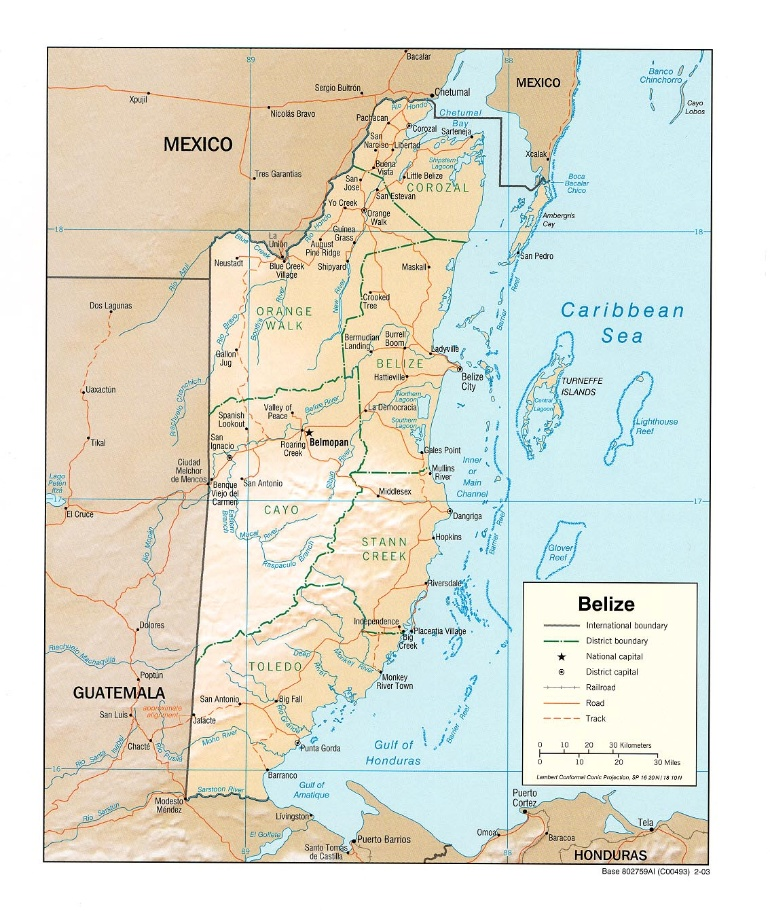
\includegraphics[width=\linewidth]{media/pap_masters_book/image4.jpeg}
\captionof{figure}{государство Белиз}
\end{minipage}

В иллюминатор самолёта персонажи видят Карибское море. Самолёт
приземляется на рассвете в аэропорту имени Филипа С. У. Голдсона
(международный код BZE). На выходе из аэропорта персонажей встречает
оперативник ``Мира и процветания'' Сергей Волков, водитель видавшего виды
грузовика с надписью на тенте <<Мир и процветание --- сила и
справедливость>>.

Грузовик отправляется на базу ``Мира и процветания'' в Бельмопан.
Чувствуется морской бриз, но по мере наступления дня становится жарко.

Примерно через полтора часа в пути грузовик проезжает блокпост <<Мира и
процветания>>, который можно узнать по флагу.

Персонажи игроков не знают и не могут этого видеть, но на блокпосте
только что прошла пересменка: БМП Marder привёз на блокпост
оперативников с базы и забрал ночную смену (1 сержант и 5 рядовых),
чтобы вернуть её на базу. БМП выезжает на шоссе как раз перед тем, как
мимо блокпоста проезжает грузовик с персонажами игроков.

Никто не подозревает, что в это время боевики Диего Ортис и Маркос
Веласкес устроили засаду именно на БМП ``Мира и процветания''. Они знают
время пересменки на блокпосте и маршрут движения. Диего Ортис
заблаговременно устанавливает на шоссе мину ТМК с радиовзрывателем, а
сами боевики маскируются в лесу, подступающему прямо к шоссе Джорджа
Прайса на полпути между Ла Демокрасиа и Бельмопаном.

Через несколько минут движения после проезда блокпоста, персонажи
игроков слышат взрыв: это мина подрывается точно под БМП. Сергей Волков
нажимает на тормоз и кричит "все из машины", после чего сам покидает
кабину.

Боевики попытаются по возможности расстрелять всех оперативников <<Мира и
процветания>> из БМП, а также Сергея Волкова, который попытается оказать
им помощь. Они не будут пытаться убить персонажей игроков, а в случае
угрозы попытаются скрыться.

Если Сергей Волков погибнет, персонажам игроков придётся самим
добираться до Бельмопана и базы ``Мира и процветания''.

Патруль ``Мира и процветания'' после взрыва мины прибудет на место атаки
минут через пять-десять, за это время нападающие успеют скрыться. Тела
убитых (если они есть) привезут на базу ``Мира и процветания'' только к
вечеру на грузовике.

Если персонажи игроков свяжутся с патрулём или солдатами на блокпосте,
то им помогут добраться до базы. Солдаты свяжутся с базой и персонажей
игроков на базе встретит Ханс Шмидт.

\subsection{Разговор с Хуаном Эстебаном Каррерой}\label{carrera-meeting}

Ханс Шмидт приказывает группе оперативников ``Мира и процветания'' прибыть
в штаб. В штабе Шмидт, Смирнов, Донской.

Ханс Шмидт говорит, что договорился о разговоре с местным торговцем
оружием, Хуаном Эстебаном Каррерой. Он знает его давно и ожидает, что
разговор пройдёт спокойно, но Шмидт не знает, с какими людьми Каррера
ведёт дела, и поэтому хочет подстраховаться, взяв с собой оперативников.
Задача оперативников: сопровождать Ханса Шмидта, быть настороже, но не
делать резких движений.

К выезду нужно быть готовыми через 2 часа.

К моменту выезда приезжает грузовик. Шмидт садится с водителем в кабину,
а оперативники вместе с персонажами игроков едут в кузове в особняк
Хуана Эстебана Карреры в Бельмопане.

По возвращению на базу оперативников распускают. Шмидт уходит в штаб,
приказывает в штаб никого не пускать. Если Каррера жив, то идёт с
Хансом.

У игроков свободное время. Солдаты, которые были с игроками, расходятся
кто в столовую, кто спать. Потом они могут уехать на другие задания.

Самый активный игрок получает +1 к ЛГК или ВЛН. Все игроки получают по 2 очка
тренированности к любым навыкам.

\subsection{Убийство Хуана Эстабана Карреры}\label{carrera-murder}

Если Хуана Эстебана Карреру доставили на базу живым, то той же ночью его
убивают прямо на базе ``Мира и процветания'' вместе со своими охранниками,
зарезав ножами, причём так, что никто этого не видел и не слышал. Тем не
менее, Каррера успевает рассказать Шмидту о том, что большую часть
оружия ему поставляет офицер армии Белиза Ахмед Хассан, а самый большой
покупатель этого оружия -- некий Рауль Мендоса. Конечно же, факт смерти
Карреры сильно огорчает весь офицерский состав ``Мира и процветания'',
ведь становится очевидно, что база -- крайне небезопасное место.

\subsection{Обнаружение схрона боевиков}\label{hideout-discovery}

Дмитрий Донской вызывает персонажей игроков в штаб. Там Шмидт и Донской.

Донской рассказывает, что ночью один из тайных патрулей <<Мира и
процветания>> заметил вооружённых людей и проследил за ними и в настоящий
момент продолжают наблюдение. Патруль запрашивает помощь для ареста.
Персонажам игроков поручается арестовать этих вооружённых людей. Прямо
сейчас предлагается обсудить детали операции и осуществить её как можно
скорее. Боевиков как минимум трое. У них видели штурмовые винтовки и
пулемёт, но, возможно, у них есть что-то ещё.

Шмидт выписывает бессрочный пропуск на выход с территории базы, а также
разрешение для получения оружия. Кроме того, он говорит, что договорился
с правительственными войсками о предоставлении в помощь грузовика с
отделением солдат (7 человек: рядовой водитель, сержант, младший
сержант, 4 рядовых, если среди них есть солдат с навыком ПЛМ,
то он получает пулемёт). Шмидт намекает, что неплохо бы взять хотя бы
одного боевика живым, чтобы допросить и узнать, кто снабжает их оружием.

Донской предлагает разделиться на два отряда и зайти с разных сторон под
прикрытием дымов. Он выбирает персонажа с наибольшим Макс(ЛГК/ВЛН) и предлагает
ему стать командиром первого отряда. Как вариант, если у персонажа со
вторым по убыванию Макс(ЛГК/ВЛН) значение Макс(ЛГК/ВЛН) больше Макс(ЛГК/ВЛН) командира отряда
белизцев, Дмитрий предлагает ему взять на себя командование белизцами.
Опционально можно выделить третий отряд и взять в него часть белизцев.
Если персонажей игроков больше 2, они могут сформировать дополнительные
отряды и действовать самостоятельно, либо быть просто солдатами отряда.
Если они простые солдаты, они перемещаются вместе с отрядом, но
действовать могут отдельно. В конечном итоге игроки сами решают, как им
сформировать отряды.

Донской приказывает идти готовиться и доложить о готовности.

Когда игроки докладывают Донскому о готовности, на базу приезжает
грузовик с белизцами. Белизцы будут выполнять только исходную задачу,
они откажутся участвовать в других событиях.

По возвращении с задания персонажей ждёт в штабе Шмидт. Он просит
рассказать о том, что произошло.

После разговора Шмидт распускает персонажей по казармам. Если игроки не
хотят оставаться в казарме, они могут пойти ночевать в гостинице, но за
свой счёт.

Самый активный игрок получает +1 к ЛГК или ВЛН. Все игроки получают по 2 очка
тренированности к любым навыкам.

\subsection{Разговор с Хосе Родригесом}\label{rodriguez-meeting}

Если к этому времени персонажи игроков не получили информацию от Хосе
Родригеса самостоятельно, то ночью игроков разыскивает Дмитрий Донской.
Он берёт персонажей игроков с собой на встречу с Хосе Родригесом в
качестве охраны.

Они отправляются в гостиницу ``Формоза''. Там они проходят в номер, где их
встречает Хосе Родригес. Он предлагает выдать интересную информацию в
обмен на протекцию и работу в ``Мире и процветании''. Донской обещает
помочь ему.

Донской благодарит Хосе, говорит, что свяжется с ним, а персонажей
игроков просит об этом пока никому не рассказывать и возвращается на
базу.

\subsection{Засада на армейский конвой}\label{army-convoy-ambush}

Правительство Белиза получает документы, из которых следует, что <<Мир и
процветание>> продаёт оружие на чёрном рынке. Также всё чаще масс-медиа
освещаются сюжеты, очерняющие компанию и подчёркивающие её неспособность
обеспечивать порядок и закон. Отношение властей Белиза к <<Миру и
процветанию>> заметно ухудшается, ``Мир и процветание'' больше не получает
помощь местных военных. Счета компании заморожены, она не может вести
хозяйственную деятельность.

Местные перестали идти на контакт, и Ханс Шмидт не может ничего выяснить
об Ахмеде Хассане и его роли в торговле оружием. Он подозревает, что
местные силовики на самом деле ведут борьбу с ``Миром и процветанием''.
Сдаваться он не собирается и решается на крайне рискованный и отчаянный
шаг: допросить Ахмеда Хассана, используя информацию, полученную от Хосе
Родригеса. Ханс понимает, что это акт войны против государства, но также
понимает, что время работает против него.

По информации от Хосе Родригеса, Конвой поедет по шоссе Хэммингберд на
юг. У персонажей игроков есть сутки на подготовку.

Шмидт приказывает Донскому организовать операцию. Донской включает
персонажей игроков в команду и вызывает в штаб на инструктаж. Там Шмидт
и Донской.

Подготовившись, персонажи игроков прибывают на лесную дорогу.
Периодически по ней проезжают гражданские автомобили. Наконец,
показывается армейская колонна. Впереди едет БТР 82 А, за ним пара
грузовиков. Ахмед Хассан сидит в бронетранспортёре. С ним 5 солдат, в
грузовиках ещё по 3 рядовых с мл. сержантом в каждом. Если у солдат есть
навык ПЛМ, то у них есть пулемёт. Если у солдат есть навык
ТВ, то у них есть РПГ-7. Если есть навык СН,
то есть снайперская винтовка.

В одной из машин 10 кг взрывчатки.

Если удастся захватить кого-то живым, это будет Ахмед Хассан. В
противном случае его без сознания можно будет найти в БТР или рядом.

Самый активный игрок получает +1 к ЛГК или ВЛН. Все игроки получают по 2 очка
тренированности к любым навыкам.

\subsection{Атака на базу националистов}\label{nationalist-base-attack}

Выявление схемы кражи оружия у ``Мира и процветания'' отчасти
стабилизирует ситуацию. Алексей Смирнов исчез, но солдат, с которыми он
работал, удалось выявить. Виктор Кравченко оказался ни при чём, его
использовали в тёмную. Однако, чтобы восстановить отношения с
правительством, нужны аргументы.

Ханс Шмидт решает провести операцию против Рауля Мендосы. Во-первых,
Рауль Мендоса может стоять за нападением на ``Мир и процветание'', а
во-вторых, его можно будет связать с армией Белиза через оружие,
доказав, таким образом, что оружие боевикам поставляет не <<Мир и
процветание>>, а армия Белиза.

Ханс Шмидт поручает проработку операции Дмитрию Донскому.

\subsubsection{Победа ``Мира и процветания''}\label{pap-victory}

Персонажи игроков успешно штурмуют базу националистов и собирают всё
оружие ``Мира и процветания'', которое могло попасть к боевикам через
Алексея Смирнова. После этого на базу националистов приглашают
следователей и чиновников Белиза.

Следствие подтверждает, что оружие боевикам было поставлено из армии
Белиза, а не передано ``Миром и процветанием''. Поддельные документы,
сфабрикованные Алексеем Смирновым, теряют вес.

Правительство Белиза размораживает счета ``Мира и процветания''. Каждому
персонажу, участвующему в штурме базы националистов выплачивается \$20
тыс.

\subsubsection{Победа наркокартеля}\label{cartel-victory}

Персонажи игроков уходят из компании ``Мир и процветание'' и
договариваются с Раулем Мендосой.

``Мир и процветание'' вынуждено сократить персонал и уйти из Белиза. Армия
Белиза сращивается с наркокартелем, и страна постепенно переходит под
теневое управление наркобарона Энрике Вальдеса.

\subsubsection{Сохранение стасус-кво}\label{status-quo}

Компании ``Мир и процветание'' не удаётся доказать свою непричастность к
торговле оружия и переложить всю вину на другую сторону.

Компания ``Мир и процветание'' вынуждена сократить персонал, персонажи
игроков не получают выплат и их увольняют. В армии и полиции проводятся
``чистки'' -- увольняют ``козлов отпущения''. Коррупция не уничтожена, но
обуздана. Наркокартель сохраняет влияние, но имеет противовес.

\section{База ``Мира и процветания''}\label{pap-base}

База ``Мира и процветания'' располагается рядом с военной базой
правительственных войск и небольшим аэропортом под названием Гектор
Сильва (международный код BCV). Находится в зоне покрытия сотовой сети.

Территория базы огорожена забором из сетки Рабица с колючей проволокой.
На базе установлено множество камер видеонаблюдения.

В восточной части находится КПП.

На базе ``Мира и процветания'' есть электронная база данных разрешений. У
всех оперативников есть электронные жетоны с идентификатором. Когда
оперативник получает разрешение, оно заносится в БД.

В юго-восточном углу территории находится стоянка с техникой, а в
северо-восточном углу ангар для техники, который соединяет со стоянкой
множество следов от гусениц и колёс. На стоянке под открытым небом стоят
бронетранспортёр и танк.

В южной стороне по центру находится ангар, в котором помещается
командный пункт. Над ним на трёх мачтах развеваются флаги компании,
Белиза и Бельмопана, а также установлены спутниковые и радиоантенны.
Перед входом в командный пункт установлена небольшая будка дежурного.

Ещё один ангар находится по центру в северной стороне, в нём находится
склад снаряжения и вооружения.

Вся западная часть территории за ангарами заставлена небольшими жилыми и
бытовыми контейнерами. Там же находится общая столовая, представляющая
из себя несколько объединённых контейнеров. Ещё одна пара объединённых
контейнеров является лазаретом, на этих контейнерах намалёваны красной
краской кресты.

\subsection{КПП}\label{checkpoint}

КПП оборудована небольшим контейнером, где находится дежурный и охрана.
Дежурный осуществляет контроль разрешений с помощью электронной БД и не
пропустит персонажей без разрешения на вход или выход. Дежурный
сменяется в 00:00, каждый день это новый человек. Дежурного можно
уговорить пропустить персонажа без пропуска. Для этого нужно пройти
проверку Макс(ЛГК/ВЛН) со сложностью 21 (бросок D20 + Макс(ЛГК/ВЛН)).
Можно дать взятку. За каждые \$100 сложность снизится на 2.

\subsection{Командный пункт (штаб)}\label{command-post}

Дежурный на входе в командный пункт контролирует доступ внутрь. Если
персонажи хотят поговорить с командованием, дежурный сначала докладывает
об этом начальству и пропускает их только если начальство даёт добро.

\subsection{Казармы}\label{base-barracks}

Казармы -- это множество небольших контейнеров.

Внутри каждого контейнера двухъярусная кровать, двухсекционный шкаф для
личных вещей, стол, два стула, немного свободного пространства. В каждом
контейнере есть душевая комната и туалет.

В некоторых контейнерах есть люди. Это персонал базы, в основном
солдаты. Они отдыхают или занимаются своими делами. В казармах они
неохотно разговаривают и просят персонажей не мешать им.

Люди периодически ходят в столовую, приезжают на базу и уезжают на
задание, перед заданием их вызывают в штаб, потом они собираются и в
какой-то момент за ними приезжает транспорт.

\subsection{Столовая}\label{base-mess}

Столовая -- это несколько контейнеров, совмещённые вместе. Люди,
находящиеся в столовой, более разговорчив, чем люди, которые отдыхают в
казармах.

\subsubsection{Слухи}\label{rumors}

С базы можно отлучиться и без разрешения, когда нет задания. Иногда
можно договориться с дежурным на КПП.

На периметре базы у камер где-то есть слепая зона, но где именно
неизвестно, а человек, который знает, сейчас на задании.

В Бельмопане в баре ``Голубая устрица'' можно выпить и снять проститутку.

В Бельмопане, в оружейном магазине ``Яблочке'' можно купить кое-какую
экипировку.

В Бельмопане на рынке можно нанять людей для грязной работы. Бригадир
Тайлер Дерден.

В Бельмопане на рынке можно достать наркотики. Дилер Тайлер Дерден.

Однажды участвовал в стычке с бандитами. Они обнюхались наркоты и
совершенно не чувствовали страх. Пёрли на пулемёт в полный рост.
Интересно, есть ли стимуляторы, которые дают такой же эффект и не
вызывают проблем со здоровьем?

К югу от Бельмопана есть нарколаборатория. Там самая дешёвая цена для
оптовых покупателей. Это недалеко от клуба каякинга, который устраивает
туры по реке через пещеры.

\subsubsection{Атака на ``Мир и процветание''}\label{pap-under-attack}

Произошло жестокое нападение на солдат ``Мира и процветания''. За
деятельное участие в расследовании обещана премия в \$20 тыс.

Никто не понимает, откуда у бандитов достаточно оружия, чтобы напасть на
БМП. Это очень тревожный сигнал.

\subsection{Лазарет}\label{infirmary}

Лазарет -- это несколько контейнеров, совмещённые вместе, поменьше, чем
столовая.

В лазарете два пациента: у одного острое отравление, понос и рвота, а
второй перенёс операцию по удалению аппендицита. За пациентами ухаживает
Александр Борода.

\subsection{Изолятор}\label{brig}

Изолятор -- это несколько контейнеров, совмещённые вместе, похожи на
лазарет, но в них нет окон и все двери закрываются снаружи. Внутри
пространство разграничено на камеры металлическими перегородками, в
каждой камере есть туалет и умывальник. Когда в изоляторе содержатся
заключённые, снаружи дежурит оперативник ``Мира и процветания''.

\subsection{Склад снаряжения и вооружения}\label{equipment-storage}

Это большой металлический ангар, внутри которого в металлических
закрытых контейнерах хранится снаряжение и оружие. На входе есть
небольшая зона, огороженная сеткой, где сидит офицер Виктор Кравченко.
На склад посетители не проходят, персонал склада выдаёт оружие со склада
через специальный тамбур.

\subsection{Стоянка техники и технический ангар}\label{vehicle-parking}

На стоянке стоят KPz Fuchs и M1A1 Abrams. В танке нет боеприпасов для
танковой пушки.

В техническом ангаре есть подъёмные механизмы и инструменты для ремонта
техники, а также склад запасных частей. Когда персонажи прибывают в
Белиз, в ангаре проходят ремонт 3 грузовика.

В ангаре постоянно находится Тони Нгуен. Он либо руководит работой, либо
сидит в отдельной каморке в углу ангара.

\subsection{Преступления персонажей}\label{character-crimes}

\subsubsection{Самовольное оставление базы}\label{unauthorized-departure}

В некоторых случаях персонажем может быть запрещено покидать территорию
базы.

Если выйти из базы через КПП, уговорив или подкупив дежурного, и
вернуться в тот же день, то о самоволке командование не узнает. Если
вернуться в другой день, дежурный сменится и не пропустит без пропуска.
Придётся его уговаривать или подкупать снова, либо он доложит о
происшествии начальству, и тогда оно узнает о самоволке.

Можно попытаться скрытно перелезть забор, для этого нужно пройти
проверку МСК со сложностью 10. Обратно нужно будет сделать то же самое.
Игроки в любом случае перелезают, но в случае успеха о самоволке не
узнают, а в случае хотя бы одной неудачи из двух -- узнают. Но это будет
понятно только по возвращении.

При возвращении на базу, если начальство ничего не узнало, то сценарий
продолжается как обычно. Если узнало, то нарушителей вызывают в
командный пункт. В штабе солдаты с оружием, требуют у виновных сдать
оружие. Ханс Шмидт материт и передаёт Дмитрию Донскому для наказания.
Персонажей игроков сильно избивают, они теряют 1 очко тренированности в
каких-нибудь навыках. Затем их оттаскивают в казармы.

\subsubsection{Арест местной полицией}\label{police-arrest}

Если полиция арестовывает персонажей, то через некоторое время передаёт
их либо в Мир и процветание, либо на местную армейскую базу в
зависимости от текущей политической ситуации.

Если персонажей игроков передают в Мир и процветание, то происходит
примерно то же самое, что и при самовольном оставлении части, но игроки
теряют 2 очка тренированности в каких-нибудь навыках и их предупреждают,
что расстреляют, если что-то подобное ещё раз повторится. Кроме того,
никто на базе больше не будет сотрудничать с игроками, только формально
и не более того.

Если персонажей передают местной армии, то персонажи будут подвергаться
унижениям. Они будут терять по 1 очку тренированности в каких-нибудь
навыках каждый день, пока очки ВНС не снизятся до 0 и персонажи не
погибнут от мучений.

\subsection{Сергей Волков}\label{sergei-volkov}

Молодой оперативник ``Мира и процветания'', около 25 лет, водитель
грузовика.

\subsubsection{Слухи}\label{rumors-volkov}

База находится в Бельмопане, рядом с военной базой правительственных
войск и небольшим аэропортом под названием Гектор Сильва.

Дорога от аэропорта Филипа Голдсона займёт около 2 часов.

Сергей Волков просит у персонажей денег в долг. Если спросить зачем, он
отвечает, что хочет купить кое-какую экипировку в магазине оружия
``Яблочко'' в городе Бельмопан. Он предлагает сходить в магазин вместе,
если будет возможность, но упоминает, что новичкам сначала нужно
получить разрешение на выход в город.

\subsection{Ханс Шмидт}\label{hans-schmidt}

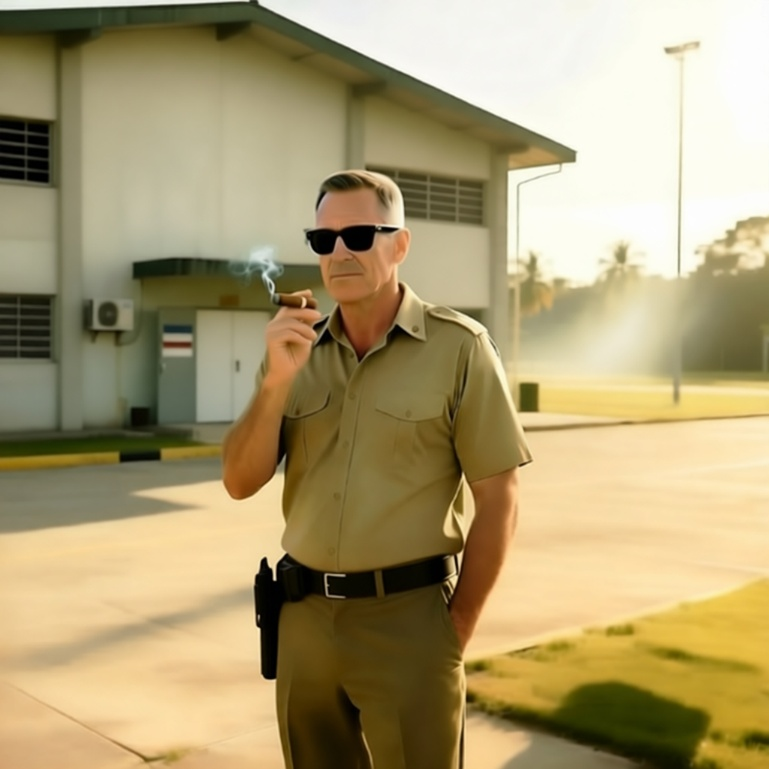
\includegraphics[width=\linewidth]{media/pap_masters_book/image5.jpeg}

Ханс Шмидт -- это подтянутый мужчина, на вид 50 лет. Он одет в рубашку
цвета хаки с коротким рукавом и брюки того же цвета. У него короткая
стрижка, он курит сигары, часто носит тёмные очки.

Шмидт имеет большой опыт работы в Белизе, работал там ещё до заключения
контракта с ``Мир и процветание''.

Шмидт встречает персонажей, когда они приезжают в Бельмопан. Он
представляется как командующий базой и представляет Алексея Смирнова,
одного из офицеров.

Ханс рассказывает, что по базе можно свободно перемещаться, обстановка
спокойная. Отлучаться с базы можно только по разрешению Смирнова или
Шмидта. База поддерживает силовые операции правительства по борьбе с
терроризмом и организованной преступностью. Сотрудники выступают
инструкторами, а также в некоторых случаях как группа быстрого
реагирования для решения сложных задач. Этим же предстоит заниматься и
персонажам. Пока они могут заселяться и обустраиваться на новом месте.

После этого Шмидт предлагает задавать вопросы. Когда вопросы исчерпаны,
Шмидт просит Алексея проводить персонажей в казармы, а сам уходит в
штаб.

\subsubsection{Слухи}\label{rumors-schmidt}

Сейчас на базе порядка 50 сотрудников ``Мира и процветания''. Помимо
этого, к операциям привлекаются солдаты правительственной армии.

Правительственную военную базу, которая находится рядом, собираются
расформировать и передать её под управление ``Мира и процветания'', тогда
условия будут более комфортабельными. Но пока она ещё действует.

Помимо Шмидта и Смирнова на базе есть офицеры Виктор Кравченко, который
отвечает за склад оружия, Тони Нгуен, который отвечает за технику, и
Дмитрий Донской, консультант-инструктор.

Оружие можно будет получить после заселения, но только стандартное:
гранаты, дымовые шашки, штурмовую винтовку. Чтобы получить что-то сверх
лёгкого стрелкового оружия и гранат, нужно разрешение Шмидта или
Смирнова. Также Шмидт может договориться о привлечении дополнительных
людей из армии Белиза или специалистов ``Мира и процветания'', но это
делается под конкретную задачу.

\subsubsection{Александр Борода}\label{alexander-beard}

Ханс Шмидт будет готов отпустить Александра Бороду из лазарета на свои
задания после смерти Карреры, до этого он отвечает, что в лазарете
Борода нужнее. Кроме того, Шмидта нужно уговорить: пройти проверку
Макс(ЛГК/ВЛН) со сложностью 10. В случае успеха, Александр присоединится к команде
на следующее задание. На задание, связанное с атакой националистов Шмидт
отпустить Александра без уговоров.

\subsubsection{Запчасти для техники}\label{vehicle-parts}

При вопросе про запчасти отсылает к Тони Нгуену.

При вопросе о деньгах на запчасти отвечает, что обычно так не делается,
запчасти заказываются через централизованную систему компании.

Если Шмидту сдали деньги за продажу неисправных гранат, он отдаст их на
ремонт техники.

Если просить деньги до обнаружения схрона боевиков, Шмидт не увидит
целесообразности самим заниматься ремонтом. Можно попытаться его
убедить, пройдя проверку Макс(ЛГК/ВЛН) на 18.

Если просить деньги после того, как правительство получит поддельные
документы, очерняющие ``Мир и процветание'', то счета будут заблокированы
и выделить деньги на ремонт будет невозможно. Шмидт сможет только дать
D4 сотен долларов на ремонт из своих личных денег.

\subsubsection{Использование исправной техники}\label{using-working-vehicles}

Ханс разрешает использовать исправную технику, которая стоит на базе
``Мира и процветания''.

\subsubsection{Атака на ``Мир и процветание''}\label{pap-attack-schmidt}

Это вызов ``Миру и процветанию''. Подобные события приводят к потере очков
компании и ставят под угрозу продление контракта и укрепление позиций
компании в Белизе. Необходимо найти тех, кто это организует и сделать
так, чтобы подобное не повторилось. Это -- основная задача на ближайшее
время для всех сотрудников ``Мира и процветания''.

За деятельное участие в расследовании этого дела назначена награда \$20
тыс.

\subsubsection{Хуан Эстебан Каррера}\label{carrera-info}

Ханс Шмидт имел дело с Каррерой, когда тот ещё служил в армии, а сам
Шмидт служил в разведке и посещал Белиз. Ханс уважительно к нему
относится, знает, что тот занимается нелегальной торговлей оружием, но
закрывает на это глаза. Шмидт не знает других контрагентов Карреры.

\subsubsection{Об интересе Рашида к гранатам}\label{rashid-grenades}

Ханс Шмидт предлагает продать Рашиду неисправные гранаты, которые
взрываются в руках пользователя, но деньги нужно будет сдать Шмидту.
Неисправные гранаты можно получить у Виктора Кравченко.

\subsubsection{События у схрона боевиков}\label{hideout-events}

Шмидт будет огорчён, если узнает, что у боевиков много тяжёлого
вооружения. Ему непонятно, откуда вдруг у бандитов такие ресурсы. У него
такое впечатление, что он воюет с армией Белиза, а не с какими-то
бандитами, пусть и организованными.

\subsubsection{Связь между Гомесом и Хассаном}\label{gomez-hassan-link}

Шмидт будет огорчён этой информацией. Это подтверждает его опасения по
поводу участия в событии армии Белиза. Он благодарит за информацию и
говорит, что ему надо подумать. Предлагает персонажам не предпринимать
самостоятельных действий по этому поводу.

\subsubsection{Связь между Гомесом и Кравченко}\label{gomez-kravchenko-link}

Шмидт будет огорчён этой информацией. Это ещё раз указывает на то, что
база ``Мира и процветания'' не является безопасным местом.

Шмидт знает, что Виктор Кравченко закупал оружие у Карреры, это было с
ним согласовано. Он не знает, продавал ли Виктор ему оружие, но без
доказательств склонен верить в лояльность Виктора.

Шмидт благодарит за информацию и говорит, что ему надо подумать.
Предлагает персонажам не предпринимать самостоятельных действий по этому
поводу.

\subsubsection{Захват Ахмеда Хассана}\label{hassan-capture}

Ситуация крайне сложная и Ханс приказывает доставить Ахмеда Хассана на
допрос, захватив его, когда тот будет вне военной базы. Это подпольная,
незаконная операция, поэтому необходимо убедиться, что нападающих нельзя
будет связать с компанией ``Мир и процветания'': переодеться и оставить
все личные вещи на базе. Об операции никому не сообщать, официально
оперативники едут патрулировать Бельмопан.

Ахмеда Хассана не следует привозить на базу ``Мира и процветания''. Нужно
его привезти на ферму ``Ранчо Гарсия'', где Ханс Шмидт сможет сам
допросить Хассана.

\subsubsection{Атака на базу Рауля Мендосы}\label{mendosa-base-attack}

Ханс Шмидт приказывает организовать и осуществить атаку на базу Рауля
Мендосы.

Необходимо арестовать или уничтожить Рауля Мендосу и убедиться, что все
улики, которые следователи найдут на месте, будут указывать на поставку
оружия из армии Белиза, а не из ``Мира и процветания''. В случае успеха
участники операции получат премию в \$20 тыс.

\subsection{Алексей Смирнов}\label{alexey-smirnov}

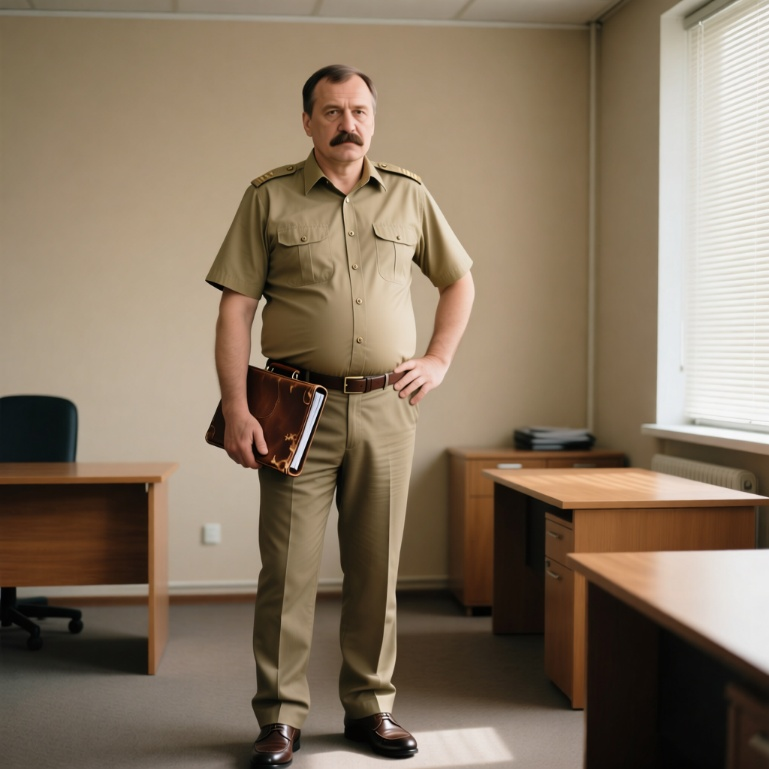
\includegraphics[width=\linewidth]{media/pap_masters_book/image6.jpeg}

Алексей Смирнов --- усатый мужчина лет 45, невысокого роста, с
небольшим, но заметным животом. Одет по форме компании <<Мир и
процветание>>: хаки-рубашка с коротким рукавом и брюки того же цвета.
Обувь начищена, все пуговицы аккуратно застёгнуты, документы в папке под
мышкой --- образ типичного штабного администратора с лёгким цинизмом в
глазах. Выглядит как надёжный и деловитый офицер, вежливый в общении.

\subsubsection{Слухи}\label{rumors-smirnov}

Мы -- коммерческая компания, мы здесь не для того, чтобы проповедовать
какие-то идеалы, а для того, чтобы зарабатывать деньги. Чем больше
заработаешь, тем раньше выйдешь на пенсию.

\subsection{Виктор Кравченко}\label{viktor-kravchenko}

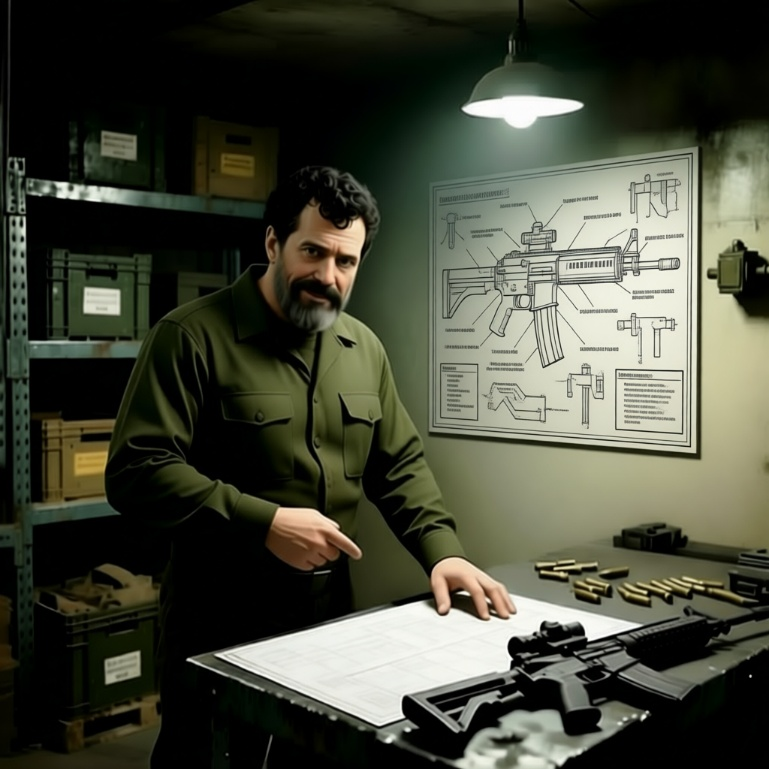
\includegraphics[width=\linewidth]{media/pap_masters_book/image7.jpeg}

Виктор Кравченко -- это мужчина 50 лет, с тёмными курчавыми волосами и
массивными чёрными усами, немного медлительный. Он постоянно находится
на складе оружия и, в свободное от работы время, любит разбирать и
чинить оружие.

Виктор Кравченко может выдать лёгкое стрелковое оружие и гранаты просто
по списку, без особых разрешений.

По разрешению Шмидта или Смирнова может выдать дополнительное снаряжение
или тяжёлое оружие из наличия.

Когда персонажи прибывают в Белиз, на складе мало оружия. Нет никаких
БПЛА, нет миномётов, нет ПТРК и ракет к ним. Нет боеприпасов к танковым
пушкам, к артиллерии. Есть один подствольный гранатомёт, гранаты к нему,
два РПГ-7 и 4 ракеты к ним. На вопрос почему нет некоторого снаряжения
Виктор отвечает, что всё разобрали.

Перед нападением на армейский конвой становится доступен ПТРК Метис-М, 4
ракеты к нему.

Перед атакой на базу Рауля Мендосы становятся доступными 2
разведывательных дрона, 2 ударных дрона с радиоуправлением, один 60 мм
миномёт, 16 мин к нему, 10 снарядов для танка.

\subsubsection{Покупка оружия у Карреры}\label{buying-weapons-carrera}

Виктор Кравченко иногда закупает у Карреры оружие и боеприпасы, потому
что по официальному каналу приходит не всё и недостаточно.

Конкретно это работает так: Кравченко заполняет заказы и передаёт их
через Алексея Смирнова. Алексей Смирнов ведёт общую бухгалтерию базы.

\subsubsection{Передача оружия бандитам}\label{weapons-to-bandits}

Если показать Виктору оружие, которое игроки нашли в логове Рашида
Гомеса, то он ответит, что да, это оружие ``Мира и процветания'', что
подпись на бумаге его, но он понятия не имеет, как оно попало к Рашиду.

Виктор Кравченко отрицает обвинения о продаже оружия боевикам. Он злится
из-за этих обвинений и перестаёт сотрудничать с персонажами, пока они не
принесут извинения.

\subsection{Тони Нгуен}\label{tony-nguyen}


\includegraphics[width=\linewidth]{media/pap_masters_book/image8.png}

Тони -- чернокожий мужчина примерно 40 лет. Хорошо знает технику. В
свободное время он любит смотреть телевизор, читать книги и газеты.

\subsubsection{Слухи}\label{rumors-nguyen}

Техники мало, исправная постоянно используется.

Заказанные запчасти очень долго приходится ждать.

\subsubsection{Техника на стоянке}\label{vehicles-parking}

Fuchs и Abrams доставили недавно, они неисправны и в причинах пока не
разбирались. Пока они не распределены по экипажам. Если видит среди
игроков механика, то намекает, что новичок может получить технику в
управление, если поможет с ремонтом.

\subsubsection{Диагностика техники на стоянке}\label{vehicle-diagnostics}

Можно уговорить Тони разобраться что с техникой, пройдя проверку Макс(ЛГК/ВЛН) со
сложностью 10. Можно пойти и посмотреть самому, пройдя проверку МЕХ
соответствующего класса со сложностью 10. В танке неисправна система
смазки, а в Fuchs неисправен рулевой механизм.

\subsubsection{Поиск запчастей для техники}\label{parts-search}

Тони знает, что запчасти могут быть на базе правительственных войск (но
официально они говорят, что нет), либо где-то в городе. Говорит, что в
полутора километрах по прямой к юго-западу от базы есть мастерская <<Край
водителя>>, где местные иногда обслуживают тяжёлую технику и вездеходы.
Рулевые тяги, теоретически, можно сделать, но для этого нужно найти
кузнеца с кузницей, а Тони не знает, где такое может быть.

Если сказать Тони, что есть запчасти за деньги, то он отвечает, что у
него денег нет, надо разговаривать с Хансом Шмидтом.

\subsubsection{Ремонт техники}\label{vehicle-repair}

Чтобы починить технику с использованием запчастей, нужно опять либо
уговаривать Тони это сделать, проходя проверку Макс(ЛГК/ВЛН) со сложностью 10,
либо чинить самим, проходя проверку на соответствующий МЕХ со сложностью
10.

\subsection{Александр Борода}\label{alexander-beard-2}


\includegraphics[width=\linewidth]{media/pap_masters_book/image9.jpeg}

Это крепкий лысоватый мужчина с пышной растительностью на щеках и
подбородке. Он в камуфляжных штанах и тельняшке.

\subsubsection{Слухи}\label{rumors-beard}

Александр говорит, что медицина -- это его крест. На самом деле ему не
интересно возиться с этими ущербными солдатами и тяготится службой в
лазарете. Он презирает их за то, что они потеряли боеспособность не на
поле боя, а из-за какой-то ерунды. На самом деле он служил в десанте и
ему в кайф выходить на операции, но, к сожалению, другого медика сейчас
на базе нет. Александр просил Ханса Шмидта заменить его, но тот не пошёл
Бороде на встречу и отвечал, что в этом нет необходимости. Александр
намекает, что, если игроки вдруг узнают о какой-нибудь ``необходимости'',
чтобы они напомнили Шмидту о Бороде, и тогда Александр Борода может
присоединиться к игрокам.

\subsection{Дмитрий Донской}\label{dmitry-donskoy}

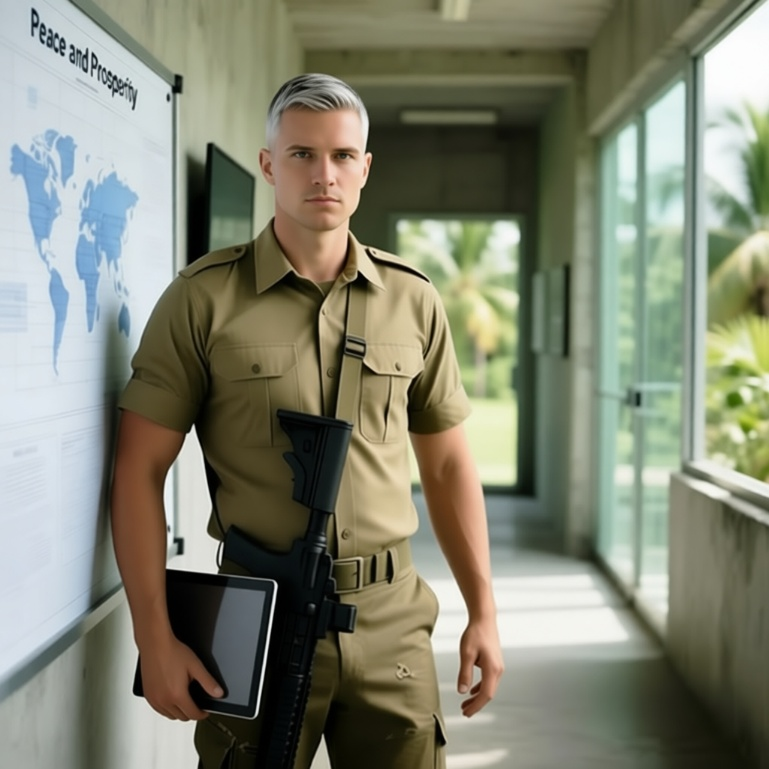
\includegraphics[width=\linewidth]{media/pap_masters_book/image10.jpeg}

Дмитрий Донской --- офицер по планированию боевых операций на базе <<Мира
и процветания>> в Бельмопане. На вид ему около 35 лет, у него коротко
стриженные седеющие виски и пронзительный, спокойный взгляд --- такой
взгляд не допускает суеты и паники. Его точные движения вызывают
невольное уважение. Носит стандартную форму компании: рубашку цвета хаки
с короткими рукавами и брюки того же оттенка. Манера общения ---
лаконичная и деловитая. Он говорит чётко, без пафоса, но с внутренней
уверенностью. Любит подчёркивать важность тактики, координации и
разведки. Прагматик, который ценит инициативу, если она обоснована и не
идёт вразрез с общей целью. Уважает тех, кто умеет думать на поле боя. В
отличие от других офицеров, носит с собой боевое оружие, а не пистолет.

\subsubsection{Атака на ``Мир и процветание''}\label{pap-attack-donskoy}

Было совершено нападение на отряд ``Мира и процветания'', когда
осуществлялась ротация на одном из блокпостов. Это неожиданно дерзкое и
жестокое нападение. Не понятно, кто мог его осуществить и какие у них
были мотивы. Однако, очевидно, что у нападавших было достаточно тяжёлого
вооружения. К сожалению, по горячим следам выследить нападающих не
удалось.

\subsubsection{Атака на конвой Ахмеда Хассана}\label{hassan-convoy-attack}

Операцию будут проводить персонажи игроков совместно с группой недавно
прибывших на базу новичков из Африки -- они точно не вовлечены в местные
дела. Это отделение в составе сержанта, мл. сержанта и 6 рядовых. У них
нет своего оружия, оружие надо получать у Виктора Кравченко.

На задании необходимо иметь противотанковое вооружение: ручные
реактивные гранатомёты, ПТРК.

Желательно выбрать место, где шоссе идёт через густой лес. Такие места
есть в 30-50 км по шоссе на юг.

У персонажей игроков сутки на подготовку.

\subsubsection{Атака на базу Рауля Мендосы}\label{mendosa-base-attack-2}

Донской говорит, что для этой операции в распоряжении игроков будет Хосе
Родригес, который теперь работает на ``Мир и процветание'', а также все
солдаты, с которыми игроки работали раньше (за исключением погибших):
африканцы, Александр Борода, а также ещё одно отделение солдат <<Мира и
процветания>>: сержант, мл. сержант и 6 рядовых.

Дмитрий предлагает сначала провести скрытную разведку. Это можно сделать
под покровом ночи, либо с использованием дронов.

Он напоминает, что следует опасаться мин.

В целом на планирование и осуществление операции отводится несколько
дней.

При обсуждении результатов Дмитрий предложил бы нейтрализовать блокпосты
с помощью миномёта.

\section{Бельмопан}\label{belmopan}

\begin{minipage}{\columnwidth}

\includegraphics[width=\linewidth]{media/pap_masters_book/image11.png}
\captionof{figure}{город Бельмопан (OpenStreetMap)}
\end{minipage}

Все локации в Бельмопане находятся в зоне действия сотовой сети.

\subsection{База правительственных войск}\label{govt-base}

База окружена бетонным забором с колючей проволокой, гораздо серьёзнее,
чем сетка Рабица на базе ``Мира и процветания''. На КПП персонажей не
пропустят.

\subsection{Мастерская ``Край водителя''}\label{drivers-edge-shop}

Мастерская ``Край водителя'' находится в Изумрудном проезде примерно в
километре к югу от базы ``Мира и процветания''. Это ровная площадка,
огороженная ветхим забором с воротами и металлическим ангаром. Нах У
ворот, а также над ангаром размещены рекламные щиты, обещающие дешёвую
замену масла, шиномонтаж и ремонт техники. Ангар открыт, внутри
подъёмники для ремонта и инструменты. Днём там работают три мастера:
Дерек Мартин, Хавьер Рамирес, Мануэль Путч.

В мастерской есть масляный насос, который подойдёт для танка Abrams, но,
чтобы его найти, нужно пройти проверку на МЕХ гусеничные БМ со
сложностью 10.

Если попытаться забрать насос, когда мастера это видят, они начнут бой.
У них есть пистолеты-пулемёты или пистолеты.

Если начать стрельбу, полиция и солдаты приедут в течение 20 мин.

\subsection{Мастерская ``Винт и болт''}\label{screw-bolt-shop}

Мастерская ``Винт и Болт'' находится неподалёку от особняка Карреры,
примерно в километре на северо-восток, на Конститьюшен Драйв.

В мастерской обслуживаются грузовики. Армейские грузовики привозят в
мастерскую ящики с оружием с военной базы армии Белиза и оставляют его.
Это оружие, которым торгует Хуан Эстебан Каррера. Впоследствии ящики
забирают другие грузовики.

Рашид Гомес отсюда забирает оружие, которое отвозит в свой схрон, после
чего его замечает патруль ``Мира и процветания'' в момент разгрузки в
схроне.

\subsection{Магазин оружия ``Яблочко''}\label{weapon-shop-yablochko}

В магазине ``Яблочко'' можно купить бинокль за \$20, дальномер \$200,
разведывательный БПЛА Mavic за \$250, пистолет за \$500, 6 дымовых шашек
за \$60, дробовик за \$300, прибор ночного видения за \$500, гидратор
\$10, тепловизионный прицел для снайперской винтовки с увеличением 12x
за \$15000, бронежилеты MSV: базовый за \$400, плиты на живот и спину за
\$200 обе, защита паха, плеч и боковые пластины за \$300.

\subsection{Бар ``Голубая устрица''}\label{blue-oyster-bar}

В баре есть проститутки разных полов (услуги -- \$100, плюс \$100 за
номер в гостинице ``Формоза'').

В баре работает бармен Эрнесто Валлес.

В баре периодически бывает Рашид Гомес до того момента, как его убьют,
арестуют или идентифицируют в схроне боевиков.

По вечерам в баре поёт Изабель Амара.

После того, как персонажи игроков поговорят с Каррерой, но до того, как
они убьют Рашида Гомеса, в баре появляется Хосе Родригес. Хосе Родригес
не появляется в баре после убийства Рашида Гомеса.

После того, как игроки убьют Рашида Гомеса, в баре появляется Эмиль
Соренсен. Его можно найти там, пока персонажи игроков не используют его
для получения запчастей для техники.

\subsection{Рынок}\label{market}

Если спросить у кого-то про работу, люди указывают на местный рынок,
предлагают спросить Тайлера.

Рынок представляет собой 5 открытых рядов, где любой желающий может
занять место и продавать товар: мясо, овощи, фрукты, изделия ручной
работы, одежду. Также в северной стороне рынка есть несколько закрытых
павильонов.

В единственном павильоне без витрин находится Тайлер Дерден.

\subsection{Павильон Тайлера Дердена}\label{tyler-den-pavilion}

Павильон находится на рынке, это единственный крытый павильон без
витрин, где не продаётся никаких вещей.

В павильоне есть стол и шкаф. В шкафу можно найти рекламные буклеты
клуба каякинга на реке Кейвс Бранч в 15 км к югу от Бельмопана, на
которых есть фото Тайлера с людьми с оружием.

В столе можно найти 20 доз наркотиков на \$2000.

Вокруг павильона и внутри находится несколько человек, похожих на
чернорабочих: 4 и 8 соответственно. У них нет оружия, но значительное
количество очков ВНС: от 12 до 20. Это люди Тайлера. Они будут
набрасываться на атакующих Тайлера с голыми руками, давая тому время,
чтобы сбежать. Драться с ними -- это состязание в ВНС. Если их убить, то
это вызовет проблемы с местными властями, с полицией, и в конечном итоге
ухудшит отношения персонажей игроков с Миром и процветанием.

\subsection{Гостиница ``Формоза''}\label{formosa-hotel}

В гостинице можно снять номер за 50 долларов. Есть конференц-залы, если
они не заняты, в них пускают бесплатно.

\subsection{Полицейский участок}\label{police-station}

Если игроки ведут себя в городе странно, то к ним подходит полиция. Если
игроки ведут себя вызывающе, их арестовывают. Если у них есть оружие, но
нет разрешения, их арестовывают в любом случае. Если начинается бой,
мгновенно приезжают солдаты с базы, которая находится неподалёку. Можно
попытаться скрыться от них, можно попытаться сдаться им. Если игроков
арестовывают, то полиция передаёт их командованию базы.

\subsection{Особняк Хуана Эстебана Карреры}\label{carrera-mansion}


\includegraphics[width=\linewidth]{media/pap_masters_book/image12.png}

Дом Хуана Эстебана Карреры находится в южной части Бельмопана. К дому
есть особый съезд с Хэммингберд Хайвей недалеко от её пересечения с
Конститьюшен Драйв. Аллея приводит к особняку с бассейном и теннисным
кортом.

В доме сам Каррера и два его охранника.

У входа в особняк находится представительный человек в тёмном строгом
костюме. Это охранник Карреры, но он вежлив и не показывает оружия. Он
идентифицирует гостей. Если гости говорят, что они из <<Мира и
процветания>>, то охранник их пропускает, в противном случае не
пропускает.

В особняке находится Хуан Каррера, обычно он находится в своём кабинете
на втором этаже. Он сидит за столом, перед ним ноутбук. Каррера работает
с ноутбуком и очевидно, что в нём есть важные сведения. Для игроков на
этом следует сделать акцент.

Если персонажи приходят в дом Карреры по заданию Ханса Шмидта или с ним,
то в момент разговора Карреру внезапно атакует снайпер, который
находится в километре южнее от особняка на склоне холма. Если снайпер
попадает, Каррера убит. После этого снайпер уходит. Если снайпер не
попадает, игра переходит в тактический режим. Каррера и его охранники в
замешательстве. Они достают оружие. Если игроки тоже в замешательстве,
то снайпер стреляет ещё раз и так пока либо Каррера не погибнет, либо
пока Каррера не будет эвакуирован, либо пока снайпер не окажется под
огнём. В последнем случае он убегает за карту. Каррера соглашается ехать
с игроками на базу ``Мира и процветания добровольно'', берёт с собой
ноутбук.

Если Каррера гибнет, то игроки могут взять с собой ноутбук или
попытаться самостоятельно его осмотреть. Если они осматривают его
самостоятельно, то видят файл ``поставки'' с датой прошлого месяца, где
видят имена с цифрами напротив каждого:

\begin{itemize}
\item
  Ахмед Хассан -\$1235.
\item
  Рик Вальс +\$580.
\item
  Виктор Кравченко +\$135.
\item
  Дерек Ву +\$220 тыс.
\item
  Изабелла Коста +\$300 тыс.
\item
  Итого \$395.
\end{itemize}

Также в кабинете Карреры есть фотографии, среди которых можно найти
Карреру вместе с Хансом Шмидтом, но на фотографии они явно моложе.

\subsection{Схрон боевиков}\label{militant-hideout}

В 8 километрах к югу от Бельмопана по Хэммингберд Хайвей находится
несколько небольших домов, окружённых лесами. В этих домах нет
постоянных жильцов.

Когда персонажи прибывают туда по заданию Ханса Шмидта, в лесу где-то в
300 м от дома находятся наблюдатели Рик Кавальери и Джон Галт. У
наблюдателей нет задачи штурмовать дом, и они не будут это делать, но
они могут поддержать штурм огнём.

Если игроки перед заданием поедут в город и проведут там более 2 часов,
то количество боевиков увеличивается. Об этом игрокам сообщат
наблюдатели.

В доме 5 боевиков (сержант и 4 рядовых, среди них пулемётчик и
гранатомётчик), а ещё 2 дополнительных (мл. сержант и рядовой), если
перед заданием игроки много времени провели в городе. Если убили
мастеров в ``Крае водителя'', то ещё плюс 2 (мл. сержант и рядовой),
причём эти начинают игру не в здании. Если игроки продали Ахмеду
гранаты, то у всех боевиков есть гранаты. Важно, чтобы у всех боевиков
было не более 3 МСК.

Если боевики чувствуют, что проигрывают бой, они могут попытаться
бросить всё оружие и бежать, так как в этом случае их скорость будет
больше, чем у нагруженных персонажей. Если им удаётся выбежать за
локацию, считается, что они скрылись. Однако, остаётся возможность
исследовать брошенное оружие.

Если удалось захватить хоть одного боевика живьём, то им оказывается
Рашид Гомес.

Если все боевики убиты, то среди трупов будет Рашид Гомес. Можно
осмотреть трупы и найти документ на имя Рашида Гомеса, пропуск на
правительственную военную базу с фотографией Гомеса, подписанный Ахмедом
Хассаном и карту, на которой отмечено место к востоку от города
Медина-Банк и написано имя Рауль Мендоса.

Игроки могут попытаться забрать оружие боевиков. Среди трупов они могут
найти РПГ-7, РПГ-29 и даже Метис. А также 5 кг взрывчатки. Если игроки
забирают какое-нибудь оружие, то в нём они находят документ о
прохождении проверки технического состояния, на котором есть эмблема
``Мира и процветания'', а также имя Виктор Кравченко.

Вскоре после того, как игроки выиграли -- дом накрывает миномётные
обстрел неизвестно откуда. Игроки должны бежать, тогда они не погибают.

Что это за обстрел -- неизвестно. Конечно же, ни правительственные
войска, ни Ханс Шмидт об этом ничего не знают.

Игроки могут вернуться на базу.

\subsection{Ферма ``Ранчо Гарсия''}\label{ranch-garcia}

Ферма находится в восточной части Бельмопана, в отдалённом районе,
примерно в 5 км от базы ``Мира и процветания''. Обычно ферма пустует.

Ханс Шмидт будет ждать на ферме после выдачи персонажам игроков задания
на атаку колонны Ахмеда Хассана. Если захватить Ахмеда Хассана живым и
доставить его на ферму, то Ханс Шмидт узнает всю информацию, которую
можно получить у Ахмеда Хассана (считается, что он автоматически
проходит проверки Макс(ЛГК/ВЛН) при допросе). После этого Ханс достаёт пистолет и
убивает Ахмеда Хассана. Он объясняет это тем, что его нельзя отпускать,
потому что он знает, кто стоит за нападением, но и арест его не принесёт
пользу компании.

Если есть другие пленные, он предлагает персонажам игроков их тоже
уничтожить, а сам возвращается на базу. Если пленные не знают, что
нападение осуществила компания ``Мир и процветание'', то при их отпуске
ничего не происходит. Если же они знают это, либо персонажи примут
решение их расстрелять, то на базе Рауля Мендосы будет больше бойцов как
раз на то количество, которое расстреляют или отпустят.

\subsection{Кузница на Санта-Мария стрит}\label{kuznitsa-santa-maria}

Кузнеца расположена на частном участке, ограниченном массивным каменным
забором. В заборе глухие металлические ворота. Днём они не заперты.

На участке большой каменный дом, двор, и каменная кузница поменьше дома,
из трубы на крыше которой днём идёт дым. Дым означает, что там работает
кузнец Эмиль Соренсен. Он оставляет широкие ворота кузницы открытыми и
из двора можно наблюдать за его работой.

\subsection{Автосалон ``Колёса судьбы''}\label{car-dealer}

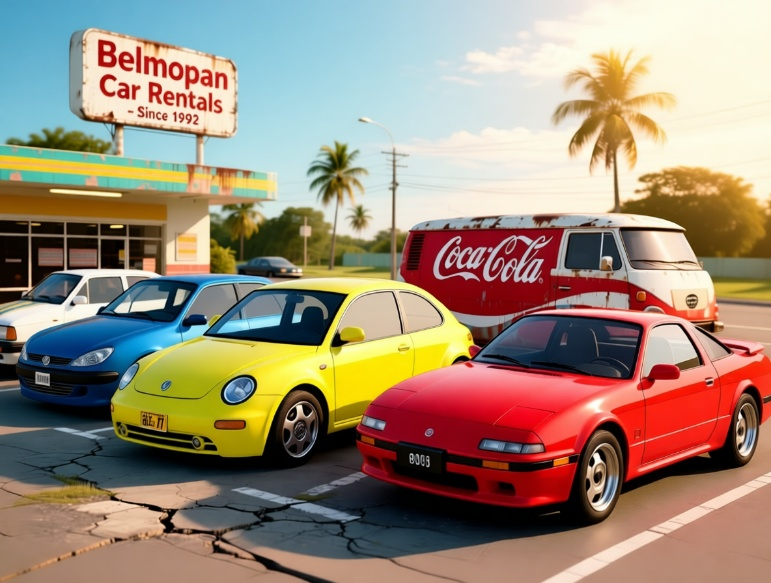
\includegraphics[width=\linewidth]{media/pap_masters_book/image13.jpeg}

Автосалон и одновременно автомойка ``Колёса судьбы'' расположена на
перекрёстке Форест Драйв и Хэммингберд Хайвей. Доступны несколько
автомобилей. Стоимость аренды \$50 в сутки.

\subsection{Рашид Гомес}\label{rashid-gomez}


\includegraphics[width=\linewidth]{media/pap_masters_book/image14.jpeg}

Рашид Гомес -- бородатый улыбчивый крепкий мужчина примерно 35 лет,
похож на турка. Предприимчивый и не лояльный к закону, сделает что
угодно, если хорошо заплатят. Мечтает сколотить собственную банду, и
добился на этом поприще некоторых успехов: у него есть связи со многими
другими легальными и нелегальными организациями. Он знаком с Раулем
Мендосой и Ахмедом Хассаном, а также связан с Энрике Вальдесом. При всём
при этом, Рашид чрезвычайно правдоподобно разыгрывает роль местного
жителя, главу большой семьи.

Рашид часто бывает в баре ``Голубая устрица'', любит вкусно поесть и
высматривает там людей, чтобы сделать бизнес или получить информацию.
Приветлив, готов пообщаться с любым.

\subsubsection{Слухи}\label{rumors-gomez}

В Белизе последнее время неспокойно, то тут, то там видят вооружённых
людей, непонятно на кого работающих. Рашид мирный житель, у него нет
оружия, он хочет защитить себя и свою семью.

Рашид хочет купить гранаты, готов заплатить \$2000.

\subsubsection{Наркотики}\label{narcotics}

Тест на Макс(ЛГК/ВЛН), может выполняться последовательно несколько раз.
Взаимодействуя с Рашидом, игрок может снизить необходимый порог для
получения информации.

При 5+ Рашид скажет, что сам не занимается и предложит обратиться к
Тайлеру Дердену.

При 10+ скажет, что может достать оптовую партию за 50\% цены, например,
для перепродажи.

При 15+ расскажет про нарколабораторию, где можно взять крупную партию
за 25\% цены.

При 20+ расскажет, что там также производится биологическое оружие.

\subsubsection{Нападение на ``Мир и процветание''}\label{pap-attack-gomez}

Всё отрицает, пока не будет взят в плен.

Рашид признаётся, что офицер с армейской базы Ахмед Хассан поручал
Гомесу осуществлять погромы и грабежи, причём хотел, чтобы они постоянно
попадали в местные новости.

Нападение на блокпосты ``Мира и процветания'' отрицает. Думает, что это
могли сделать националисты под руководством Рауля Мендосы, которые живут
неподалёку от города Медина-Банк, которым он доставлял оружие.

\subsubsection{Доставка оружия}\label{weapons-delivery}

Расскажет только если взять его в плен.

Рашид признаётся, что люди, связанные с наркокартелями, поручали ему
доставлять оружие Раулю Мендосе. Но Рашид не должен был их упоминать.

\subsection{Хуан Эстебан Каррера}\label{juan-carrera}


\includegraphics[width=\linewidth]{media/pap_masters_book/image15.jpeg}

Хуан Эстебан Каррера -- седой мужчина 65 лет. Живёт в личном особняке в
Бельмопане на Хамменгберд Хайвей. Бывший офицер армии Белиза, занимался
логистикой и снабжением. Знаком с Хансом Шмидтом, в прошлом их связывала
совместная работа в Белизе.

Уволился из армии, после увольнения участвует в нелегальной торговле
оружием. Ведёт дела со всеми, кто готов поставлять оружие и кто готов
его покупать, не интересуется моральной стороной вопроса и делами своих
контрагентов.

\subsubsection{Слухи}\label{rumors-carrera}

Каррера относительно лояльно относится к персонажам игроков. Конечно, он
не будет ничего рассказывать им, но может продать любое оружие.

\subsubsection{Торговля оружием}\label{arms-trading}

Каррера расскажет о своих делах только Хансу Шмидту и только после
покушения. Он покупает оружие у Ахмеда Хассана, а продаёт, помимо
Виктора Кравченко, ещё нескольким людям, но не знает о них ничего. Он
даже не уверен, что их имена реальны.

\subsection{Изабель Амара}\label{isabel-amara}

Изабель -- прекрасная молодая девушка, примерно 25 лет. Она --
племянница Рауля Мендосы, но об этом она не рассказывает. Она знает о
взглядах Рауля Мендосы и разделяет их, часто бывает у него на базе.

Она охотно познакомится с персонажами и ей понравится любой активный
персонаж, который захочет с ней общаться. Она будет охотно принимать
ухаживания.

\subsubsection{Слухи}\label{rumors-isabel}

Коррумпированное правительство паразитирует на стране и народе.

Военные погрязли в коррупции и озабочены только тем, как бы занять
лучшее место у кормушки.

``Мир и процветание'' -- ничем не лучше других, а только хуже, потому что
чужаки и вообще не имеют никакой связи с Белизом.

\subsubsection{Вербовка}\label{recruitment-isabel}

Активный персонаж может использовать обаяние, чтобы убедить Изабель в
том, что ``Мир и процветание'' будет служить Белизу верой и правдой. Тогда
Изабель расскажет, что её отец занимается электроникой, в том числе
военной.

Если расспрашивать её далее, то выяснится, что она может достать
детонаторы (таймер и радио) и разведывательный БПЛА. Можно купить их
(\$100 за детонатор, \$300 за БПЛА).

Если продолжать ухаживания за Изабель, то можно добиться, чтобы она
передала снаряжение бесплатно. При этом Изабель будет просить персонажа
уволиться из ``Мира и процветания'' и присоединиться к Раулю Мендосе,
который находится в местечке Майя Грин Форест неподалёку от города
Медина-Банк.

\subsection{Хосе Родригес}\label{jose-rodriguez}

Хосе Родригес -- молодой мл. сержант белизской армии. У него смуглая
кожа и вьющиеся чёрные волосы.

\subsubsection{Слухи}\label{rumors-rodriguez}

Хосе не удовлетворяет зарплата, а кроме того, у него конфликт с местными
из-за того, что он переспал с чужой женой. Он считает, что в компании
``Мир и процветание'' сможет заработать больше и заодно решить свои личные
вопросы.

\subsubsection{Вербовка}\label{recruitment-rodriguez}

Хосе Родригес хочет работать в ``Мир и процветание'', поэтому, как только
он узнает, что персонажи игроков там работают, он будет проявлять
инициативу.

Хосе хочет узнать условия работы и как происходит набор сотрудников. Он
будет благодарен, если игроки разузнают это для него и помогут ему
попасть в компанию, взамен он может предоставить информацию о базе
правительственных войск.

Хосе может достать 5 кг взрывчатки и взрыватели: на выбор таймер или
радио.

Хосе может достать один снаряд для танка или одну противотанковую мину.

Когда Родригес будет уверен, что его возьмут в ``Мир и процветание'', он
расскажет, что много раз видел, как другие солдаты белизской армии
получали оружие и экипировку от солдат ``Мира и процветания''. Также он
знает, что это оружие доставляли на армейскую базу, а затем вывозили в
другое место. Хосе не знает куда, но уверен, что об этом знает интендант
Ахмед Хассан.

Также Хосе Родригес выдаст план движения армейского конвоя, в котором
будет Ахмед Хассан: поедет по шоссе Хэммингберд на юг днём следующего
дня в известный час.

\subsection{Тайлер Дерден}\label{tyler-derden}


\includegraphics[width=\linewidth]{media/pap_masters_book/image16.jpeg}

Тайлер Дерден -- местный наркодилер и по совместительству бригадир
неквалифицированной рабочей силы. Среднего роста, худощавый, в рубашке и
джинсах. Обитая на дне, он каким-то образом удерживается от того, чтобы
полностью утонуть.

Тайлер не склонен ввязываться в смертельные сражения, он склонен убегать
от опасности с помощью своего окружения.

\subsubsection{Заработать денег}\label{earn-money}

Тайлер предлагает подработать грузчиком. Работа заключается в том, чтобы
пройти проверку на ВНС со сложностью 20, но её можно проходить сколько
угодно раз, пока она не будет пройдена. Оплата -- \$100, но это можно
делать только раз в день.

\subsubsection{Нанять людей}\label{hire-people}

У Тайлера можно нанять людей, одного человека за \$100 в день. Это будет
гражданский уровня рядовой без оружия. Если попросить этого человека
поучаствовать в военизированных операциях, он запросит \$300 сверху.

\subsubsection{Наркотики}\label{narcotics-tyler}

Тайлер продаёт дозу за \$100.

При прохождении проверки Макс(ЛГК/ВЛН) 10+ Тайлер может рассказать, что наркотики
производит местный наркокартель. Тайлер может назвать местонахождения
лаборатории, где он забирает товар.

При прохождении проверки Макс(ЛГК/ВЛН) 15+ Тайлер предупредит, что там глушат
связь, а в церкви водятся демоны.

\subsection{Ахмед Хассан}\label{ahmed-hassan}

Ахмед Хассан -- офицер армии Белиза, интендант военной базы в
Бельмопане. Среднего роста, в военной форме, носит бороду и усы.

\subsubsection{Слухи}\label{rumors-hassan}

Ненавидит ``Мир и процветание'' и всех, кто связан с компанией, так как
дорожит своим местом в армии Белиза и боится потерять положение в
обществе и пенсию.

\subsubsection{Торговля оружием}\label{arms-trading-hassan}

Если пройти проверку Макс(ЛГК/ВЛН) 20, Ахмед расскажет, что вёл дела с Алексеем
Смирновым из ``Мира и процветания''. Алексей Смирнов подписывал фиктивные
разрешения на выдачу оружия, подкупал солдат, которые потом передавали
оружие солдатам армии Белиза, а те, в свою очередь, передавали это
оружие Ахмеду. Ахмед же продавал его Хуану Эстебану Каррере, который
перепродавал его на рынке.

\subsubsection{Нападения на ``Мир и процветание''}\label{pap-attacks-hassan}

Не признаёт, что нападал на ``Мир и процветание'', хотя и одобряет это
нападение, потому что ``Мир и процветание'' ничем не лучше, так как напали
на самого Ахмеда.

Если пройти проверку Макс(ЛГК/ВЛН) 20, Ахмед расскажет, что за нападением на <<Мир
и процветание>> может стоять Рауль Мендоса, националист-террорист. Ахмед
встречался с ним однажды в местечке Майя Грин Форест неподалёку от
города Медина-Банк.

\subsubsection{Энрике Вальдес}\label{enrique-valdes}

Если пройти проверку Макс(ЛГК/ВЛН) 20, Ахмед расскажет, что это местный
наркобарон. Ахмед не знает, как его найти, но от него приходили люди и
просили передать оружие Рашиду Гомесу для передачи кому-то ещё.

\subsection{Эмиль Соренсен}\label{emil-sorensen}

Эмиль Соренсен -- добродушны весельчак, полный, с рыжими волосами и
бородой, много пьёт и говорит.

\subsubsection{Слухи}\label{rumors-sorensen}

Эмиль -- кузнец и делает холодное оружие, а также всякие изделия из
металла.

\subsubsection{Рулевые тяги для бронетранспортёра}\label{apc-steering-tie-rods}

Эмиль готов изготовить рулевые тяги для бронетранспортёра. Для этого
нужно будет сделать чертёж (проверка МЕХ колёсные БМ со сложностью 15) и
заплатить \$300. Он предложит пойти с ним на Санта-Мария стрит, где его
мастерская, и буквально через пару часов отдаст готовые рулевые тяги.

\subsection{Мастера в ``Краю водителя''}\label{mechanics-drivers-edge}

\subsubsection{Слухи}\label{rumors-mechanics}

Ещё один мастер, который работал в мастерской, продавал наркотики, а
недавно сам умер от передоза наркотиков.

Наркокартели -- это транснациональные корпорации, такие же как <<Мир и
процветание>>, только действуют вне закона.

\subsubsection{Масляный насос для Abrams}\label{oil-pump-abrams}

Да, вам повезло, такими танками пользовалась армия Белиза и примерно год
мы купили партию списанных танков с демонтированным оружием. Масляный
насос есть, отдадим его за \$2000.

\subsection{Эрнесто Валлес}\label{ernesto-valles}

Потрёпанный мужчина с седеющими волосами и шрамом над бровью. Всегда в
белой рубашке и фартуке. Движения медленные, но точные.

Это не просто бармен, а владелец бара ``Голубая устрица''.

Эрнесто не вмешивается в дела посетителей, пока не начинается стрельба.
Он видел много дерьма.

\subsubsection{Еда и выпивка}\label{food-drink}

Выпивка стоит от \$5 до \$20 за бокал. Еда --- \$10 за порцию.

\subsubsection{Слухи}\label{rumors-bartender}

Говорят, в Белизе начали пропадать люди.

Говорят, в Майя Грин Форест завёлся Робинг Гуд.

Говорят, в пещерах на реке Кейвс Бранч открылся портал в ад.

Говорят, демоны поселились в старой церкви у пещер на реке Кейвс Бранч.

Говорят, в Бельмопане становится всё больше наркоманов. Они трутся на
рынке вокруг Тайлера Дердена.

Говорят, у Белиза два пути: торговля оружием и наркотиками.

Некоторые люди надеются, что ``Мир и процветание'' решит проблемы Белиза,
а некоторые считают, что проблем станет только больше.

\section{Майя Грин Форест}\label{maya-green-forest}

Майя Грин Форест -- это деревня в джунглях неподалёку от города
Медина-Банк в южной части Белиза. Находится вне зоны действия сотовой
сети.

Там находится заброшенная школа и несколько домов, где живут Рауль
Мендоса и его люди, а также их жёны и дети. Школа оборудована подвалом,
который полностью защищает от дронов и миномётного обстрела. Из подвала
ведёт подземный ход длиной около 15 см, выход из которого замаскирован и
находится в лесополосе. Чтобы обнаружить ход, нужно пройти проверку МСК
15+, находясь в радиусе 5 см от него.

Деревня охраняется двумя блокпостами (с АГС и крупнокалиберным
пулемётом) и четырьмя патрулями по два человека. На каждом блокпосту и в
каждом патруле есть мл. сержант и рядовой. На блокпостах есть РПГ и
ракеты к ним. Около одного из блокпостов в 10 см от него на дороге
установлена противотанковая мина ТМ. Кромка леса около склада
боеприпасов заминирована минами ПФМ по линии длиной 10 см. В каждом
отряде есть дробовик для защиты от дронов.

Один из сараев является складом боеприпасов. У боевиков есть БТР-80, он
припаркован рядом со складом боеприпасов. Если подорвать склад
взрывчаткой, то БТР будет уничтожен. Экипаж БТР не сидит в нём, он сидит
в хижине: ест или спит. Однако, когда он чует неладное, тут же бежит к
машине. Теоретически, БТР может угнать персонаж с хорошим навыком МЕХ
колёсные БМ.

В школе находятся Рауль Мендоса, и его помощники, Маркос Веласкес и
Диего Ортис, если они к тому моменту ещё живы, а также ещё одно
отделение пехоты (сержант, мл. сержант и 6 рядовых). Кроме того, там
могут быть дополнительные бойцы в зависимости от того, что произошло на
ферме ``Ранчо Гарсия''.

На складе боеприпасов и в школе есть винтовки, пулемёты и станковые
пулемёты, АГС, разведывательные дроны, много взрывчатки,
радиодетонаторы, ПТРК, реактивные гранатомёты, ракеты к ним.

Если персонажи нападут на базу, там будет Изабель Амара. Женщины и дети,
находящиеся в Майя Грин Форест безоружны, но в случае боя вступаются за
своих мужчин и поднимают их оружие, если те погибают в бою.

\subsection{Рауль Мендоса}\label{raul-mendoza}

\subsubsection{Слухи}\label{rumors-mendoza}

Армия и правительство коррумпированы, и ``Мир и процветание'' ничем не
лучше, а даже хуже, потому что они только работают в Белизе, но не
живут. Он предлагает персонажам игроков посмотреть вокруг: на хуторе с
людьми Рауля жёны и дети, а кто на базе ``Мира и процветания'', кто на
военной базе Бельмопана? Рауль хочет реального мира и процветания. Он
предлагает персонажам игроков присоединиться к нему или уехать из
страны.

\subsubsection{Источник оружия}\label{weapons-source}

Оружие Раулю безвозмездно передают разные хорошие и уважаемые люди,
патриоты страны. Рауль считает, что они от чистого сердца помогают ему
бороться за справедливость.

Чтобы переубедить Рауля, убедить его в том, что оружие ему поставляет
наркокартель через Рашида Гомеса нужно пройти тест на Макс(ЛГК/ВЛН) 15+. В
этом случае Рауль может прекратить сопротивление.

\subsubsection{Рашид Гомес}\label{rashid-gomez-mendoza}

Да, он передавал Раулю оружие.

\subsubsection{Атака на ``Мир и процветание''}\label{pap-attack-mendoza}

Да, нападение на блокпост ``Мира и процветания'' осуществляли люди Рауля.

\subsubsection{Вербовка}\label{recruitment-mendoza}

Рауль и его люди могут присоединиться к персонажам игроков для борьбы с
наркокартелем. Если Рауль убеждён, что оружие поставлял картель, то 5+.
Если не убеждён, то 10+.

\section{Лабораторный комплекс}\label{laboratory-complex}

Нарколаборатория находится в 15 км к югу от Бельмопана неподалёку от
моста через реку Кейвс Бранч, через который пролегает Хэммингберд
Хайвей. Рядом находятся пещеры: пещера святого Германа, Кристальная
пещера. Находится в зоне действия сотовой сети.

Нарколаборатория представляет собой основной производственный корпус,
замаскированный под склад сельскохозяйственной техники и несколько
небольших построек. Рядом расположена небольшая церковь, а в её подвале
находится биологическая лаборатория, где создают биологическое оружие.
Нарколаборатория и биологическая лаборатория связаны между собой
подземным ходом, но в нём крайне надёжная герметичная металлическая дверь. Её можно открыть,
использовав любой компьютер в нарколаборатории или биолаборатории, пройдя проверку навыка
электроника 10+, либо взорвать взрывчаткой, противотанковой миной или снарядом для реактивного
гранатомёта. Для этого потребуется навык работы со взрывчатыми веществами 3+ и какой-нибудь
снаряд с бронебойностью 3+.

И в производственном корпусе, и в церкви установлены станции радиоэлектронных помех класса Капюшон.

В производственном корпусе можно найти 20 кг наркотиков на 2 млн
долларов. Также там находится заведующий нарколаборатории Эмилио Варгас.

Если оперативники ``Мира и процветания'' прибывают на лабораторный
комплекс и охране не удаётся их остановить, то Варгас пытается сбежать на своём автомобиле, предварительно
предупредив Энрике Вальдеса по телефону. Вальдес вышлет группу для
эвакуации наиболее ценных ресурсов нарколаборатории, которая прибудет через 1 час.

Если Варгас успеет сбежать до прибытия оперативников, в производственном
корпусе можно использовать любой компьютер и, пройдя проверку навыка электроника с порогом 10+
найти пропуск на имя Эмилио Варгас с фотографией и номером автомобиля.

Рабочие нарколаборатории также могут сообщить имя Эмилио Варгаса,
если их допросить, а также могут использовать компьютер и показать его пропуск, если их
попросить (проверка Макс(ЛГК/ВЛН) 10+).

Если игроки узнают имя Эмилио Варгаса, то можно будет объявить его в розыск и его арестуют в течение суток.
Если игроки узнают номер машины Варгаса, то его арестуют в течение пары часов.
Игроки смогут допросить его и при желании конвоировать в изолятор ``Мира и процветания''.

Охрана лабораторного комплекса: 2 отделения охраны нарколаборатории, 2
расчёта станции РЭП, 4 патруля по два человека, 2 рабочих в
нарколаборатории. Все отряды имеют радиостанции класса Акведук.

Биологическая лаборатория состоит из собственно лаборатории, а также
изолятора, в котором 10 отсеков-клеток, где содержатся похищенные люди.

В лаборатории работает заведующий Артур Крон и пара его ассистентов. В
изоляторе находятся несколько заключённых из тех похищенных людей, что
остались в живых. Некоторые ждут своей очереди, некоторые инфицированы.
Отсеки-клетки пронумерованы от 1 до 10. В восьми камерах заперты
существа, являющиеся прототипами изменённого бойца. Крон называет их
``неудачами'' --- это результаты экспериментов с разными дозировками и
составами стимуляторов, и каждый из них немного отличается от остальных.
Если кто-то из них вырвется из клетки, он будет атаковать всех подряд.
У них нет оружия, они атакуют конечностями с огромными когтями, которые в игре
работают как дробовик, но только в ближнем бою. В двух оставшихся камерах ещё находятся живые
люди --- похищенные для экспериментов, но ещё не подвергнутые воздействию.

Управление клетками осуществляется через компьютер Артура Крона. Можно
использовать его, пройдя проверку навыка электроника 10+. После прохождения
навыка персонаж игрока должен будет решить какие клетки открывать
(номера от 1 до 10). При прохождении проверки навыки электроники 20+ игроки
смогут воспользоваться системой видеонаблюдения в изоляторе. При прохождении
проверки навыка электроники 30+ игроки получат доступ к системе видеонаблюдения
всего лабораторного комплекса.

Вход в биолабораторию охраняет отделение спецназа, но отвечает только за
биолабораторию, нарколаборатория ему не важна.

\subsection{Эмилио Варгас}\label{emilio-vargas}

Мужчина 50 лет, химик-технолог. Циничен, мотивирован только деньгами.
Отвечает за закупку прекурсоров, контроль качества наркотиков и
управление рабочими в производственном корпусе.

\subsubsection{Слухи}\label{rumors-vargas}

В церкви находится вход в подземную биологическую лабораторию. Там есть
что-то очень ценное (пытается заманить персонажей игроков в ловушку).

Смотрящий по лаборатории Хавьер Моралес. Но его сейчас нет.

\subsubsection{Энрике Вальдес}\label{enrique-valdes-vargas}

Рассказывает местонахождение особняка Энрике Вальдеса.

\subsection{Артур Крон}\label{arthur-kron}

Мужчина 60 лет, бывший военный учёный. Отвечает за создание
биологического оружия.

Крон не общителен, даже скрытен. Он одержим своими разработками. Видит
цель --- не видит препятствий, он даже не замечает жутких вещей, которые
творятся в его лаборатории.

\subsubsection{Похищения людей}\label{kidnapping}

Я не знаю, что это за люди. Может, это добровольцы. Я с ними не
разговариваю, их привозят другие люди. Все вопросы к Хавьеру Моралесу.

Если попросить Артура выпустить людей, Артур откроет клетки, но он
откроет все клетки, в том числе и клетки с ``неудачами''. Те немедленно
начнут всех убивать, а Артур немедленно попытается сбежать.

\subsubsection{Наркотики}\label{narcotics-kron}

Я про это ничего не знаю. Я занимаюсь настоящей наукой. Разрабатываю и
тестирую боевые стимуляторы. Например, чтобы боец мог продолжать
выполнять задачу даже после ранения, чтобы он был невосприимчив к
стрессу. По поводу лицензий все вопросы к Хавьеру Моралесу.

\section{Особняк Энрике Вальдеса}\label{enrique-valdes-mansion}

Находится на юго-западной окраине города Пунта-Горда в 200 км езды от
Бельмопана на юг, в зоне действия сотовой сети. Подъезд к особняку
контролируется блокпостами, это закрытая зона. Снаружи это не особо
заметно, но территория оборудована скрытыми охранными средствами:
камерами с автоматическим распознаванием изображения, различные
электронные датчики.

Двухэтажный особняк в колониальном стиле, построенный из местного камня
и бетона. Стены усиленные, с скрытыми амбразурами для обороны. Крыша
плоская, с парапетом --- может использоваться как наблюдательный пункт.
Окна с бронированными стёклами, решётками с внутренней стороны.

На первом этаже находятся три зала: холл, библиотека, столовая с
отдельной кухней. В особняке в целом роскошная мебель. В холле картины,
маски майя на стенах. В кухне запасы провизии на 2 недели.

В библиотеке скрытая панель --- вход в подземный бункер. Под полом
библиотеки есть тайник с наличными, \$50 тыс.

На втором этаже расположен кабинет Вальдеса, комната связи, жилые
помещения и балкон.

В кабинете Вальдеса есть тайный ход по винтовой лестнице в подземный
бункер. В кабинете есть сейф, который можно взломать проверкой
электроники на 20+ или взорвать взрывчаткой. В сейфе данные о
нарколаборатории (доказательства связи нарколаборатории с Вальдесом),
данные о биолаборатории (доказательства похищения людей и разработки
биологического оружия, сведения о местонахождении лаборатории и ключи
для прохода в неё), а также доказательства поставок оружия Раулю
Мендосе.

В комнате связи находятся станция РЭР класса Леер-2, а также станция
спутниковой связи класса Аурига.

В подземном бункере хранится запас золота и наличных на общую сумму
\$200 тыс. и резервные копии данных на физических автономных носителях.
Из бункера к частной пристани в искусственной бухте ведёт подземный ход
длиной более 1 км. От этого хода есть замаскированный выход в джунгли в
200 м от особняка.

Энрике Вальдес в зависимости от времени суток находится в жилой комнате,
либо в своём кабинете.

Охрана лабораторного комплекса: 2 отделения охраны, расчёт станции РЭР,
4 патруля по два человека. Все отряды имеют радиостанции класса Акведук.
На крыше особняка АГС и ПТРК.

\subsection{Энрике Вальдес}\label{enrique-valdes-char}

Мужчина 52 лет, среднего роста, плотного телосложения. Предпочитает
дорогую гражданскую одежду светлых тонов (лен, хлопок). Всегда спокоен,
говорит тихо, но уверенно. Носит золотое кольцо с печаткой с
изображением семейного герба. Уроженец Белиза.

Вальдес является лидером международного наркокартеля. Уровень его
влияния так велик, что по факту его можно назвать ``серым кардиналом''
Белиза. У Вальдеса есть свои люди в правительстве Белиза и во многих
организациях, работающих на территории Белиза. Он весьма недоволен
приходом в Белиз ``Мира и процветания''.

\subsubsection{Вербовка}\label{recruitment-valdes}

Предлагает персонажам присоединиться к нему. Предлагает на месте по \$50
тыс. каждому наличными, плюс по \$500 тыс. каждому в течение суток, плюс
по \$100 тыс. каждый месяц зарплату.

\subsubsection{Рауль Мендоса}\label{raul-mendoza-valdes}

Идеалист. Я уважаю его патриотизм, но мы не партнёры. Он борется за
суверенитет, я --- за бизнес. Наши пути не пересекаются.

Успешное состязание Макс(ЛГК/ВЛН). Я финансировал его через Гомеса. Оружие
шло от Хассана. Мендоса не знает, кто платит, думает, что это народная
поддержка. Он нужен был для дестабилизации власти, чтобы вы ушли из
страны.

\subsubsection{Наркотики}\label{narcotics-valdes}

В Белизе много проблем, люди ищут забвения. Я предоставляю качественный
продукт. Это внутренний рынок, других стран не касается.

Успешное состязание Макс(ЛГК/ВЛН). Раскрывает местонахождение
нарколаборатории.

\subsubsection{Рашид Гомес}\label{rashid-gomez-valdes}

Местный предприниматель. Глава семьи, уважаемый человек.

Успешное состязание Макс(ЛГК/ВЛН). Мелкая сошка, курьер. Он доставлял
оружие.

\subsubsection{Ахмед Хассан}\label{ahmed-hassan-valdes}

Значимый член общества, офицер армии Белиза. Мы встречались по вопросам
безопасности. Он патриот, как и я, считает, что чужаки в Белизе не
нужны.

Успешное состязание Макс(ЛГК/ВЛН). Он поставлял краденое оружие.

\subsubsection{Алексей Смирнов}\label{alexey-smirnov-valdes}

Не знаю такого.

Успешное состязание Макс(ЛГК/ВЛН). Наслышан о нём, он хорошо на нас
поработал и заслужил благодарность. Именно благодаря ему <<Мир и
процветание>> понесла потери.

\subsubsection{Хавьер Моралес}\label{javier-morales}

Хороший человек, на него можно положиться.

Успешное состязание Макс(ЛГК/ВЛН). Это мой партнёр, моя правая рука.

\subsubsection{``Мир и процветание''}\label{pap-valdes}

Временщики. Вы нарушаете баланс сил. Я просто защищаю интересы страны от
транснациональной экспансии. Вам лучше уехать добровольно.

Успешное состязание Макс(ЛГК/ВЛН). Мы организовали нападения на ваши
блокпосты. Смирнов подделал документы о вашей торговле оружием. Цель ---
разрыв контракта с правительством. Вы угрожаете моему бизнесу. Впрочем,
я найду способ договорится с вашими хозяевами так или иначе. Бизнесмены
всегда поймут друг друга.

\subsubsection{Биологическое оружие}\label{biological-weapons}

Частные медицинские исследования. Инновации для сельского хозяйства и
медицины. Повышение длительности и уровня жизни. Все лицензии оформлены
правильно.

Успешное состязание Макс(ЛГК/ВЛН). Это ответ на угрозы его бизнесу со
стороны других, более мощных группировок и стран. В том числе и таких
как США и ``Мир и процветание''. Раскрывает местонахождение биологической
лаборатории и как попасть внутрь. Разрабатываются химические вещества
для использования в оружии, например, в минах, бомбах, гранатах. В том
числе можно шантажировать противников, используя мирных жителей. Кроме
того, разрабатываются специальные средства для повышения возможностей
бойцов: стимуляторы, снижающие болевой порог, увеличивающие силу,
скорость реакции, ловкость, ускоряющие регенерацию, повышающие
агрессивность, изменяющие свойства живых тканей. Отдельно исследуются
способы продлевать жизнь, лечить хронические заболевания. Все эти
технологии не только нужны самому Вальдесу. Некоторые из них он
собирается поставлять на экспорт.

\subsubsection{Похищение людей}\label{kidnapping-valdes}

Клевета. Все участники экспериментов --- добровольцы из бедных районов.
Они подписали контракты и получили компенсацию.

Успешное состязание Макс(ЛГК/ВЛН). А что делать? Для работы нужен
материал. База данных у меня в сейфе. Кто-то из них может быть ещё жив,
они содержатся в биологической лаборатории.

\subsubsection{Открыть сейф}\label{open-safe}

При успешном прохождении состязания Макс(ЛГК/ВЛН) даёт электронный ключ от
сейфа.

\end{multicols}

\clearpage

\section{Характеристики персонажей}\label{character-stats}

\begin{longtblr}[
  caption={Персонажи истории},
  label = {characters},
  note{1}={\footnotesize Если в таблице указан прочерк, то экипировка определяется уровнем: у гражданских нет ничего; у военных есть винтовка или другое оружие, которое подходит им по навыкам; у механиков-водителей пистолет-пулемёт; у штабных офицеров пистолет.}
]{
  hlines,
  row{odd}={fg=navy},
  row{even}={fg=black},
  colspec={Q[c,m,co=1]Q[c,m,co=1]Q[c,m,co=2]Q[c,m,co=2]}
}
\SetCell{c,m} Имя & \SetCell{c,m} Уровень & \SetCell{c,m} Особые навыки & \SetCell{c,m} Экипировка\TblrNote{1} \\
Ростислав Харченко & Сержант & --- & --- \\
Яков Шутов & Гражданский & --- & --- \\
Леонард Кучин & Гражданский & 2 ВНС & --- \\
1-й ассистент сержанта & Мл. сержант & 20 ЛС & --- \\
2-й ассистент сержанта & Рядовой & 6 МЕД & --- \\
Смертвич Дрэнг & Сержант & --- & --- \\
Роман Иванов & Капитан & 13 МСК, 5 ДРН & --- \\
Сергей Волков & Мл. сержант & 7 МЕХ & --- \\
Диего Ортис & Капитан & 8 МСК, 13 ВЗР, 5 ЛС, 5 ТВ & Штурмовая винтовка, РПГ-7, дымовые шашки, осколочные гранаты, мина ТМК, дробовик \\
Маркос Веласкес & Капитан & 8 МСК, 5 ЛС, 13 ПЛМ & ПКМ, дымовые шашки, осколочные гранаты \\
Ханс Шмидт & Полковник & --- & --- \\
Алексей Смирнов & Майор & --- & --- \\
Виктор Кравченко & Капитан & 8 ЛС, 8 ПЛМ, 8 ТВ & --- \\
Тони Нгуен & Лейтенант & 13 МЕХ & --- \\
Дмитрий Донской & Капитан & --- & --- \\
Александр Борода & Мл. сержант & 4 МЕД & --- \\
Хуан Эстебан Каррера & Майор & --- & --- \\
Охранники Карреры & Сержант & --- & Пистолет-пулемёт \\
Снайпер 1 & Мл. сержант & 7 СН & Снайперская винтовка \\
Снайпер 2 & Рядовой & --- & --- \\
Рашид Гомес & Сержант & 3 ГРН, 3 МСК & --- \\
Стрелок Рашида & Мл. сержант & 1 МСК & --- \\
Гранатомётчик Рашида & Мл. сержант & 3 ТВ, 1 УР, 1 ГРН, 1 МСК & РПГ-7, РПГ-29, Метис \\
Пулемётчик Рашида & Мл сержант & 3 ПЛМ, 1 ГРН, 1 МСК & Ручной пулемёт \\
Тайлер Дерден & Руководитель отдела & 14 ВЛН & --- \\
Мастера в ``Крае водителя'' & Специалист, прораб & 8 ВЛН; 13 МЕХ, 3 ЛС & Пистолет-пулемёт, пистолет \\
Рик Кавальери & Мл. сержант & 13 МСК & --- \\
Джон Галт & Мл. сержант & 13 МСК & --- \\
Водитель & Рядовой & 3 МЕХ & --- \\
Ахмед Хассан & Лейтенант & --- & --- \\
Джереми Эскобар & Рядовой & 3 МЕХ & Пистолет-пулемёт \\
Эдуардо Рамирес & Рядовой & 3 ТВ & Пистолет-пулемёт \\
Хосе Родригес & Мл. сержант & --- & --- \\
Рауль Мендоса & Майор & --- & Дробовик \\
Артур Крон & Майор & 16 МЕД, 12 ЛС, 7 ГРН & Пистолет, химические гранаты \\
Эмилио Варгас & Майор & 14 ВЛН, 12 ЛС & 2 пистолета, осколочные гранаты \\
Энрике Вальдес & Полковник & 17 ВЛН & --- \\
Неудача №1 & Рядовой & 20 ВЛН, 20 ВНС, 20 МНВ, 20 МЕД, 10 ЛС & Дробовик \\
Неудача №2 & Рядовой & 20 ВЛН, 20 ВНС, 20 МНВ, 10 ЛС & Дробовик \\
Неудача №3 & Рядовой & 20 ВНС, 20 МСК, 20 МЕД, 10 ЛС & Дробовик \\
Неудача №4 & Рядовой & 20 ВНС, 20 МСК, 10 ЛС & Дробовик \\
Неудача №5 & Рядовой & 20 ВЛН, 20 ВНС, 20 МНВ, 10 ЛС & Дробовик \\
Неудача №6 & Рядовой & 20 ВЛН, 10 ВНС, 10 МНВ, 20 ЛС & Дробовик \\
Неудача №7 & Рядовой & 10 ВЛН, 10 ВНС, 10 МНВ, 20 МСК, 10 ЛС & Дробовик \\
Неудача №8 & Рядовой & 20 МСК, 20 ЛС & Дробовик \\
\end{longtblr}

\end{document}